\chapter{Signal Prediction and Systematics}

\section{Introduction}

The predicted number of signal events is found by applying the selection cuts to
the signal MC. Corrections need to be made relating to the difference between
the photon efficiency in data and MC and to account for pile-up. In addition to
these corrections uncertainties on the signal prediction need to be determined.
These include statistical errors and systematic errors. Given that 10,000 events
are available for each signal point, the statistical error is small. It is the
systematic error on which attention must be focussed. \\

Many pieces of information goes into the calculation of the signal prediction 
and each of these pieces of information has an uncertainty associated with it. 
To evaluate the systematic error the key components need to be established: 
those that if varied within their uncertainties could cause a significant 
difference in the signal prediction. Cuts are made on jets, photons, HT and MET.
For the jet and HT cuts the jet energy scale and jet energy resolution are the
major sources of uncertainty. For the photons the main sources of uncertainty
are the photon efficiency and the pile-up. Both the HT and MET distributions are
also affected by pile-up.

\section{Photon Efficiency}

The photon efficiency needs to be determined to calculate the signal efficiency.
The photon efficiency could be found using the MC, but that relies heavily on
the correct modelling of the shower shape, isolation and other variables which
may not be well modelled in the MC. The photon efficiency should be measured
from data. In the absence of any pure photon sample in the data, electrons from 
$Z\rightarrow ee$ events are used. This relies on the similarity in detector 
response between electrons and photons. A scale factor to correct the MC photon
efficiency to the real photon efficiency in data is obtained using the
electrons (Equation \ref{eq:Scale_Factor}). \\

\begin{equation}
\epsilon_{\gamma}^{data} = \frac{\epsilon_{e}^{data}}{\epsilon_{\gamma}^{MC}}
\times \epsilon_{\gamma}^{MC}
\label{eq:Scale_Factor}
\end{equation}  

Where:
\begin{itemize}
\item $\epsilon_{\gamma}^{data}$ = photon efficiency in data;
\item $\epsilon_{\gamma}^{MC}$ = photon efficiency in MC;
\item $\epsilon_{e}^{data}$ = electron efficiency obtained using $Z\rightarrow
ee$ events in data that satisfy the photon selection; 
\item $\epsilon_{e}^{MC}$ = electron efficiency obtained using $Z\rightarrow ee$
events in MC that satisfy the photon selection. 
\end{itemize}

The selection critrea for electrons are the same as those for photons except 
that electrons have a track. The distribution in photon or electron 
identification variables is the similar for isolated photons and electrons. 
Using $Z\rightarrow ee$ events in data, the tag-and-probe method is used to find
the electron efficiency. One electron (tag) is selected with stringent criteria 
to be sure that it is an electron. Another electron (probe) with looser 
requirements is located such that the invariant mass of the two electrons lies 
in the Z peak. \\

The scale factor is found to be $\epsilon_{e}^{data}/\epsilon_{e}^{MC} =
0.953\pm 0.014(stat.)$ for events with at least one jet. Four possible sources
of systematic uncertainty on this number were considered. \\

{\bf Electrons and photons behave differently in MC:} Both electrons and photons
give EM showers in the ECAL and the selection cuts have been chosen to be
similarly efficient for electrons and photons. However, one can imagine that
there may be a slight difference between the two e.g. because of bremsstrahlung.
To check this effect the MC electron efficiency from $Z\rightarrow ee$ events
was compared with the MC photon efficiency from $\gamma$+jet events. Half the
difference between the two results, 0.5\%, was taken as a systematic error on
the scale factor. \\

{\bf Pile-up:} The MC may not accurately model the data in a high pile-up
environment. To estimate the size of this effect the scale factor was calculated
for events with fewer than 5 primary vertices and events with at least 5 primary
vertices. The number 5 was chosen because that is approximately where the 
distribution of primary vertices in the data peaks. The difference between the
scale factors in the two samples, 0.024, was taken as a systematic error on the 
scale factor. \\

{\bf }

Combining the systematic errors above with the statistical error yields a final
data-MC efficiency scale factor of $\epsilon_{e}^{data}/\epsilon_{e}^{MC} =
0.953\pm0.038$.

\section{Jet Energy Scale}

Jets are reconstructed from energy deposits in the calorimeters. $\pT$ and
$\eta$ dependent jet energy corrections are applied to the raw calorimeter 
energy to get the jet energy. Any variation in these corrections would change 
the jet $\pT$, the $\HT$ and the $\MET$. \\

The appropriate jet energy corrections are determined from $\gamma$+jet events
in data. The photon is well measured and the event is balanced (within the
$\MET$ resolution). Details of the procedure to determine the jet energy 
corrections and their uncertainties are given in \cite{jec}. This corresponds to
$\sim 3\%$ uncertainty on jets above $50\GeV$ and $\sim 5\%$ uncertainty on 
smaller jets and unclustered energy. Figure \ref{fig:JEC_vs_pT_And_Eta} shows 
the jet energy correction factors as a fucntion of jet $\pT$ for jets with 
($|\eta| = 1.0$) and as a function of $\eta$ for jets with $\pT = 200 \GeV$ (the
core of the jet distribution). \\

\begin{figure}
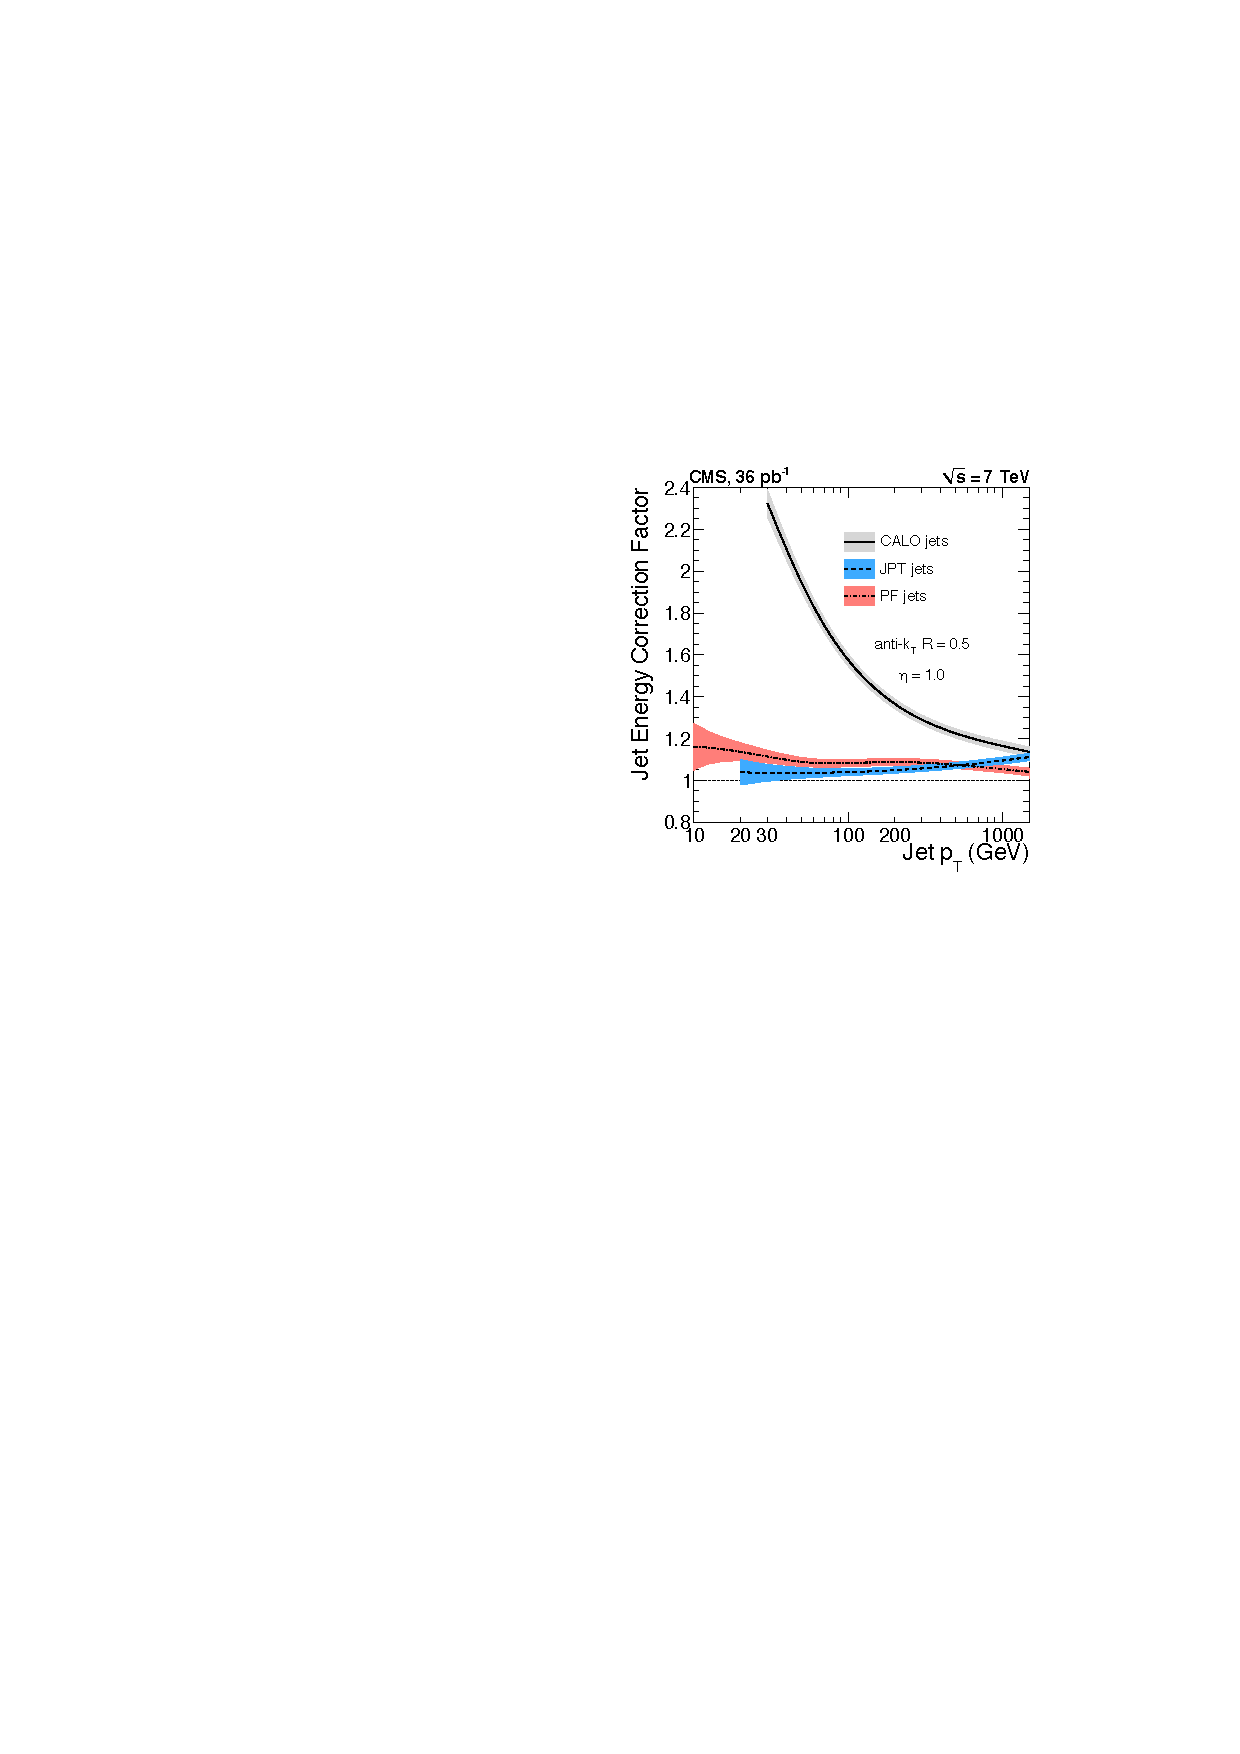
\includegraphics[width=0.5\textwidth]{JEC_vs_pT.pdf}
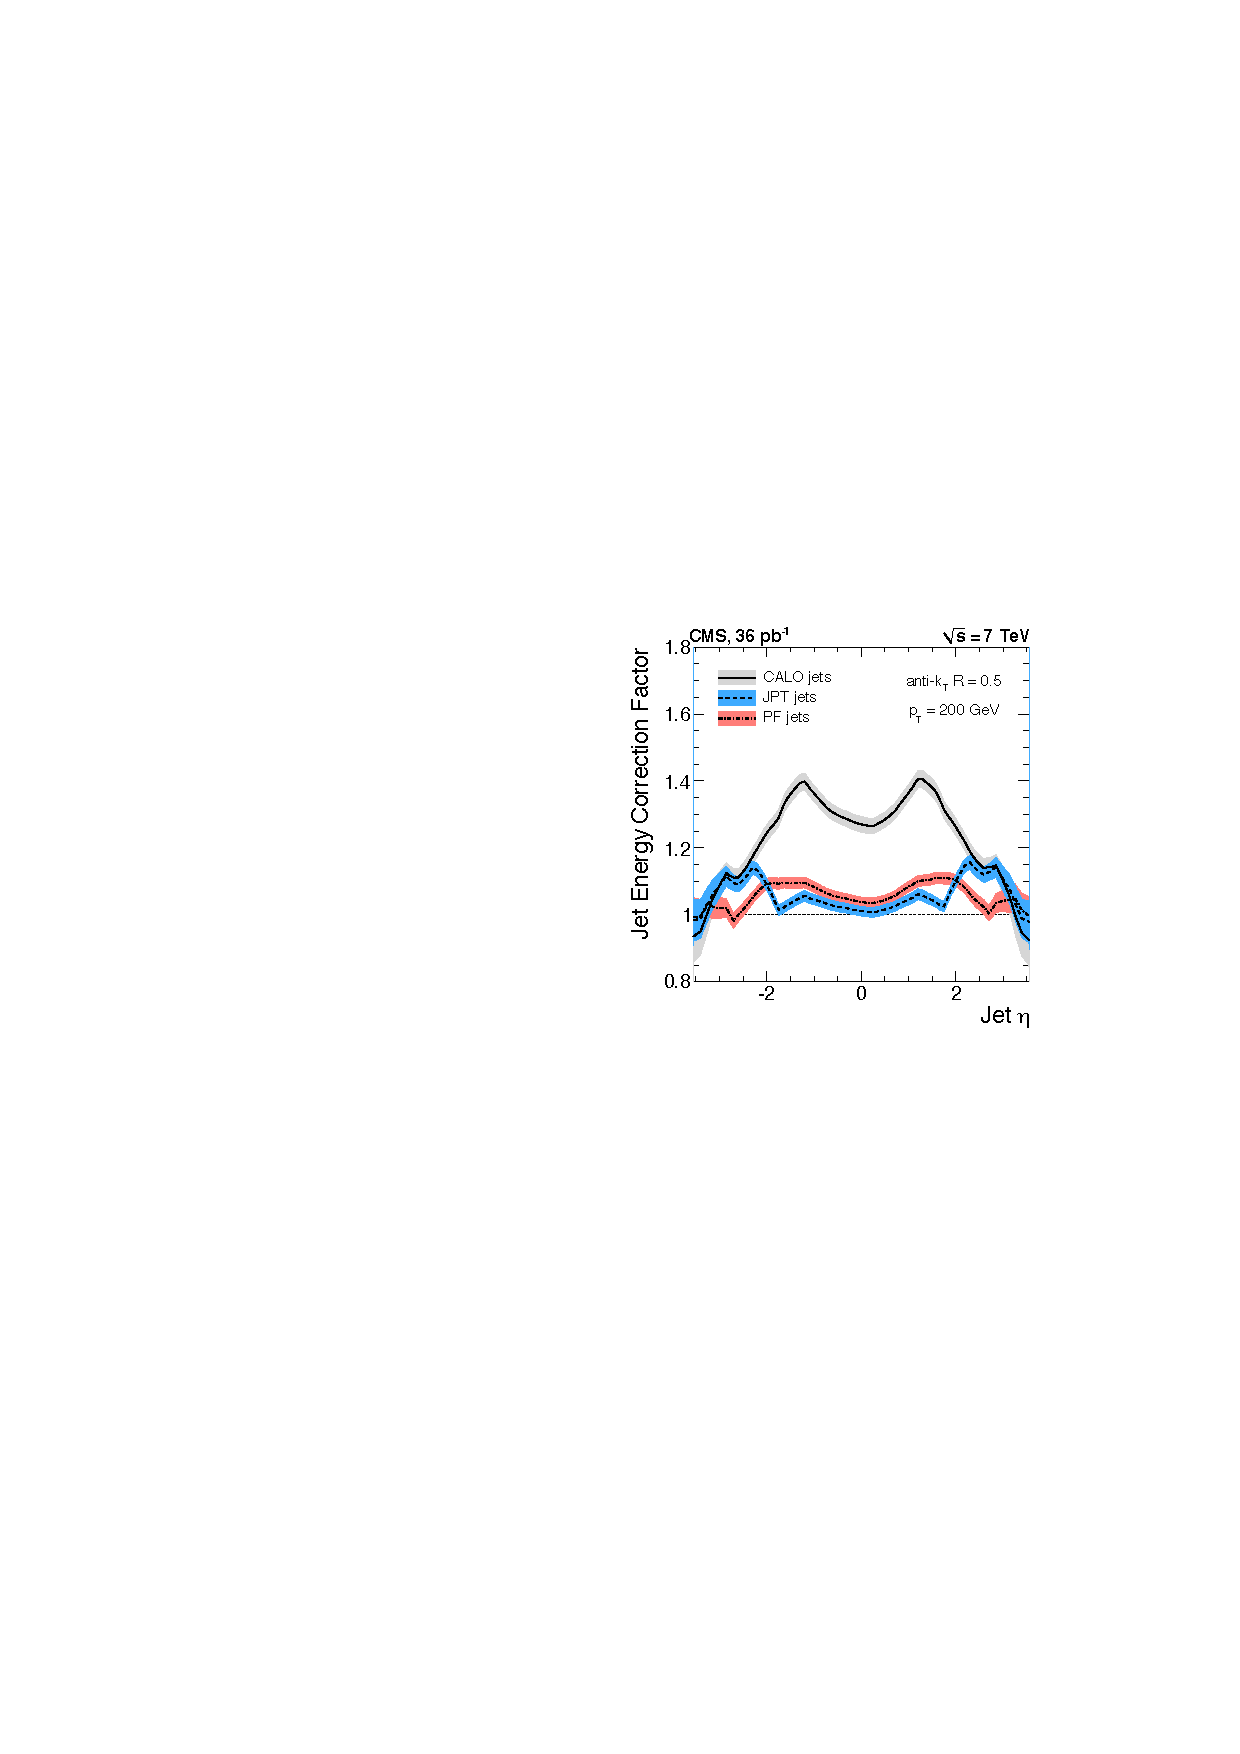
\includegraphics[width=0.5\textwidth]{JEC_vs_Eta.pdf}
\caption{The jet energy correction factor as a function of $\pT$ with $\eta =
1.0$ (left) and as a function of $\eta$ with $\pT = 200 \GeV$ (right). Three
diferent jet reconstructions are shown: CALO, JPT and PF. PF jets are used in
this analysis. The bands indicate the corresponding uncertainties.}
\label{fig:JEC_vs_pT_And_Eta}
\end{figure}

Figure \ref{fig:JES_Uncertainty_vs_Jet_pT} shows the total jet energy scale 
uncertainty against jet $\pT$ for central jets. \\

\begin{figure}
\begin{center}
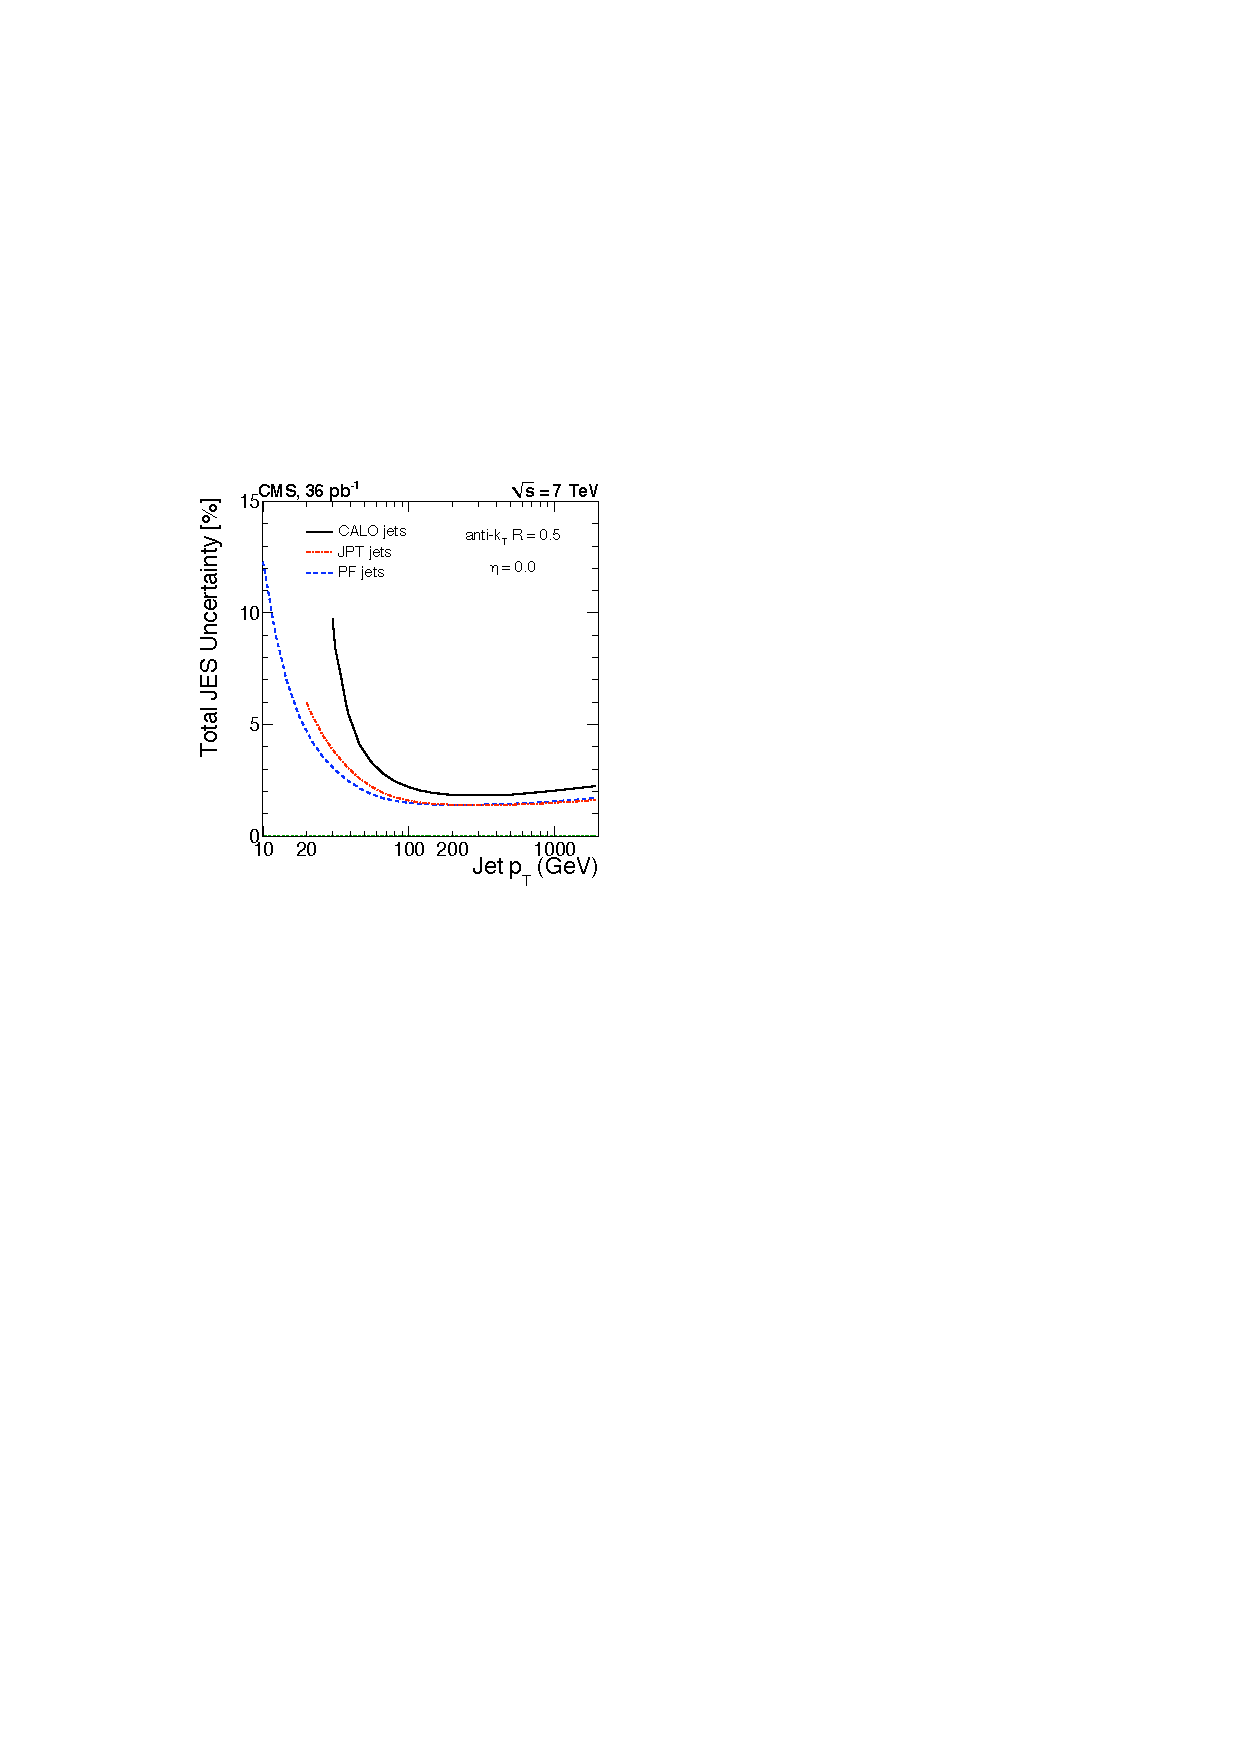
\includegraphics[width=0.7\textwidth]{JES_Uncertainty_vs_Jet_pT.pdf}
\end{center}
\caption{The total jet energy scale uncertainty as a function of $\pT$ for
central jets. Three diferent jet reconstructions are shown: CALO, JPT and PF. 
PF jets are used in this analysis.}
\label{fig:JES_Uncertainty_vs_Jet_pT}
\end{figure}

The jet energy scale uncertainties have no impact on the background estimation
because that is determined through a data-driven method. However the effect on
the number of expected signal events needs to be evaluated. \\

The $\pT$ of all the jets is modified upward and downward according to the jet 
energy uncertainties before applying the event selection. The $\MET$ can be 
expressed as Equation \ref{eq:MET}.

\begin{equation}
\MET = -\Sigma \mbox{ jets} - \mbox{photon} - \mbox{unclustered energy}
\label{eq:MET}
\end{equation}

The $\MET$ is modified to take account of the jet energy correction
uncertainties by the following procedure. 

\begin{itemize}
\item Add the photon to the $\MET$ (i.e. remove it from consideration).
\item Add the jets also to get the unclustered energy.
\item Modify the unclustered energy by 5\%.
\item Subtract the jets scaled according to the jet energy correction 
uncertainties.
\item Subtract the photon to get the modified $\MET$.
\end{itemize}

Figure \ref{fig:JES_Jet_pT} shows the leading jet $\pT$ distribution with a one 
sigma upward variation and a one sigma downward variation in jet energy scale. 
Figure \ref{fig:JES_MET_And_HT} shows how the variation in jet energy scale 
affects the $\MET$ and $\HT$ distributions. \\

\begin{figure}
\begin{center}
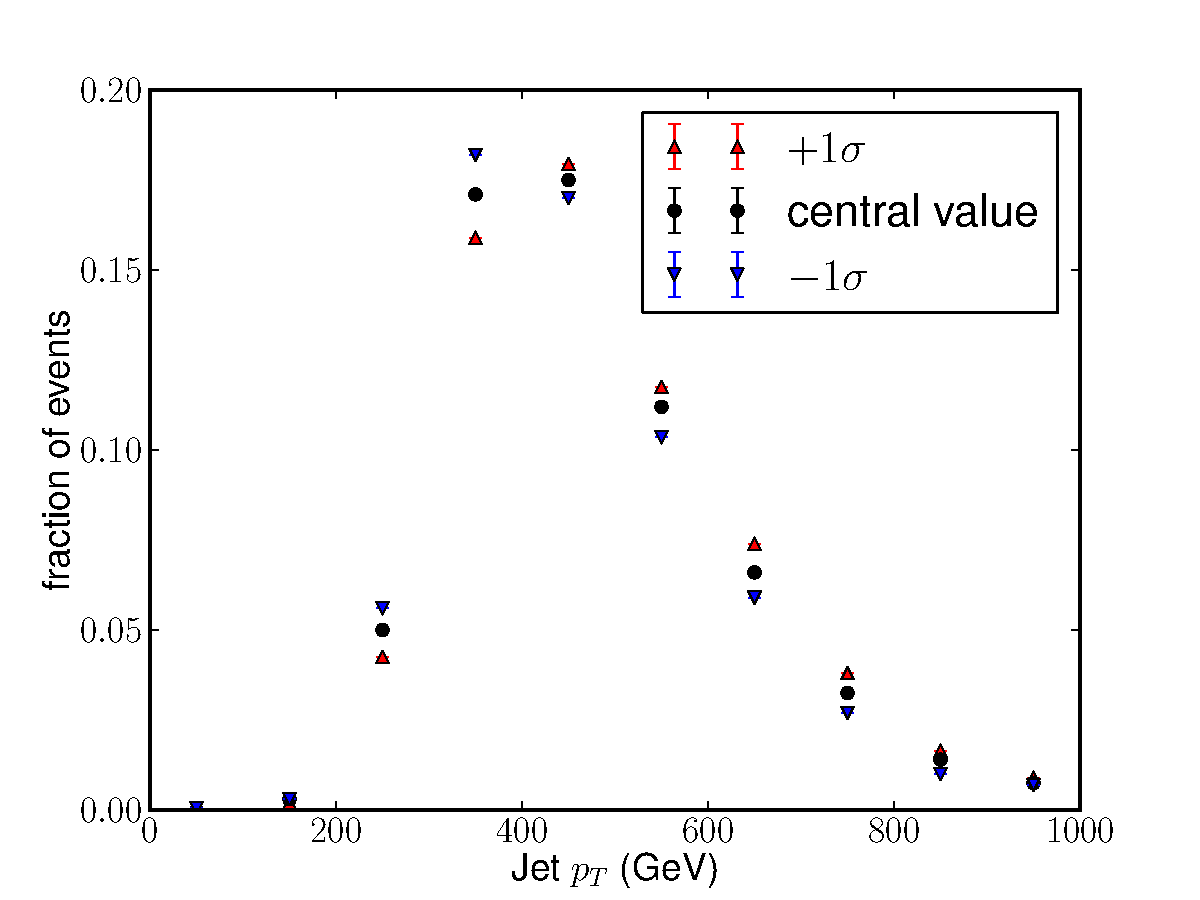
\includegraphics[width=0.7\textwidth]{JES_Jet_pT.pdf}
\end{center}
\caption{The leading jet $\pT$ distribution in signal events with a one sigma
upward variation (red) and one sigma downward variation (blue) in jet energy
scale.}
\label{fig:JES_Jet_pT}
\end{figure}

\begin{figure}
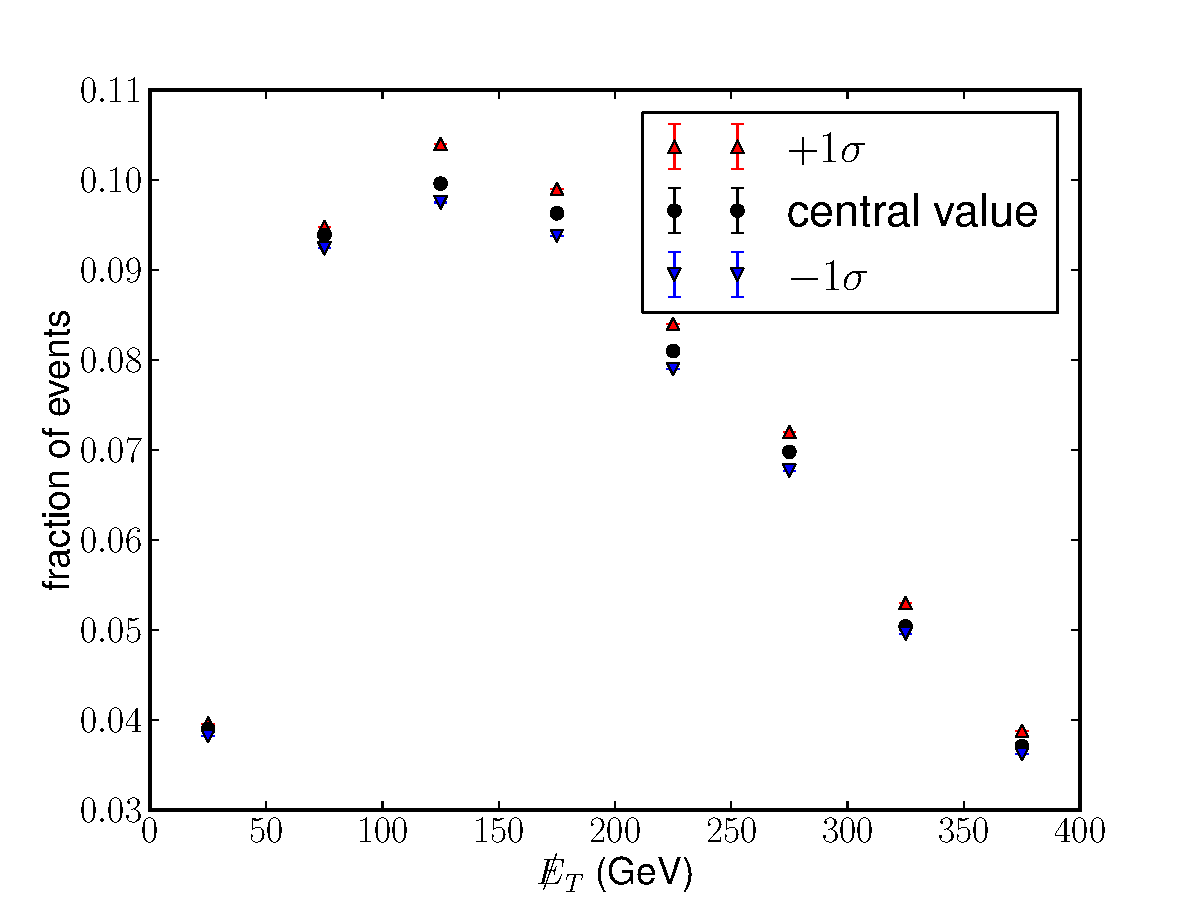
\includegraphics[width=0.5\textwidth]{JES_MET.pdf}
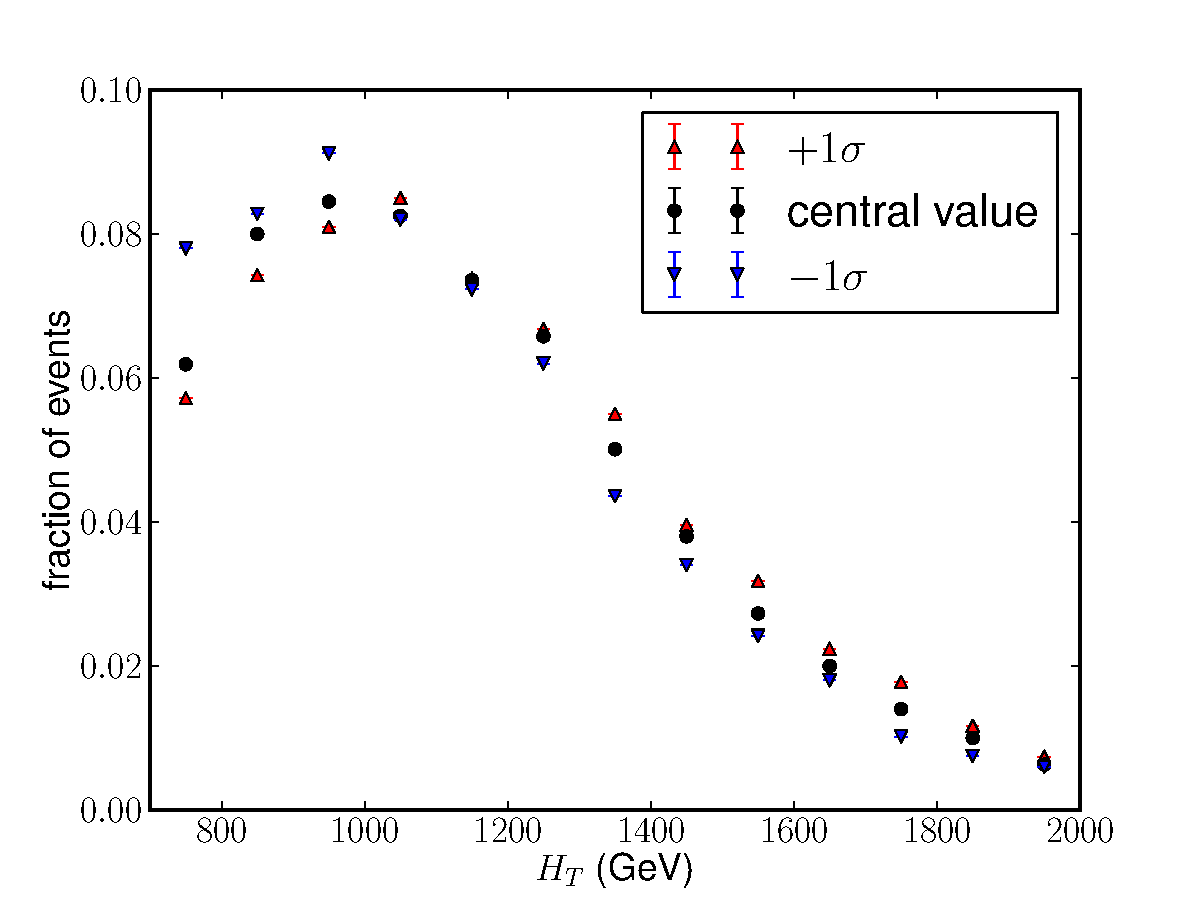
\includegraphics[width=0.5\textwidth]{JES_HT.pdf}
\caption{The $\MET$ distribution (left) and $\HT$ distribution (right) in signal
events with a one sigma upward variaton (red) and one sigma downward variation
(blue) in jet energy scale.}
\label{fig:JES_MET_And_HT}
\end{figure}

The important result is how the variation in jet energy scale affects the signal
efficiency in each ($\HT$, $\MET$) bin. Figure \ref{fig:JES_Numbers} shows these
numbers. The jet energy scale uncertainties are correlated across all 
($\HT$,$\MET$) bins.

\begin{figure}
\begin{center}
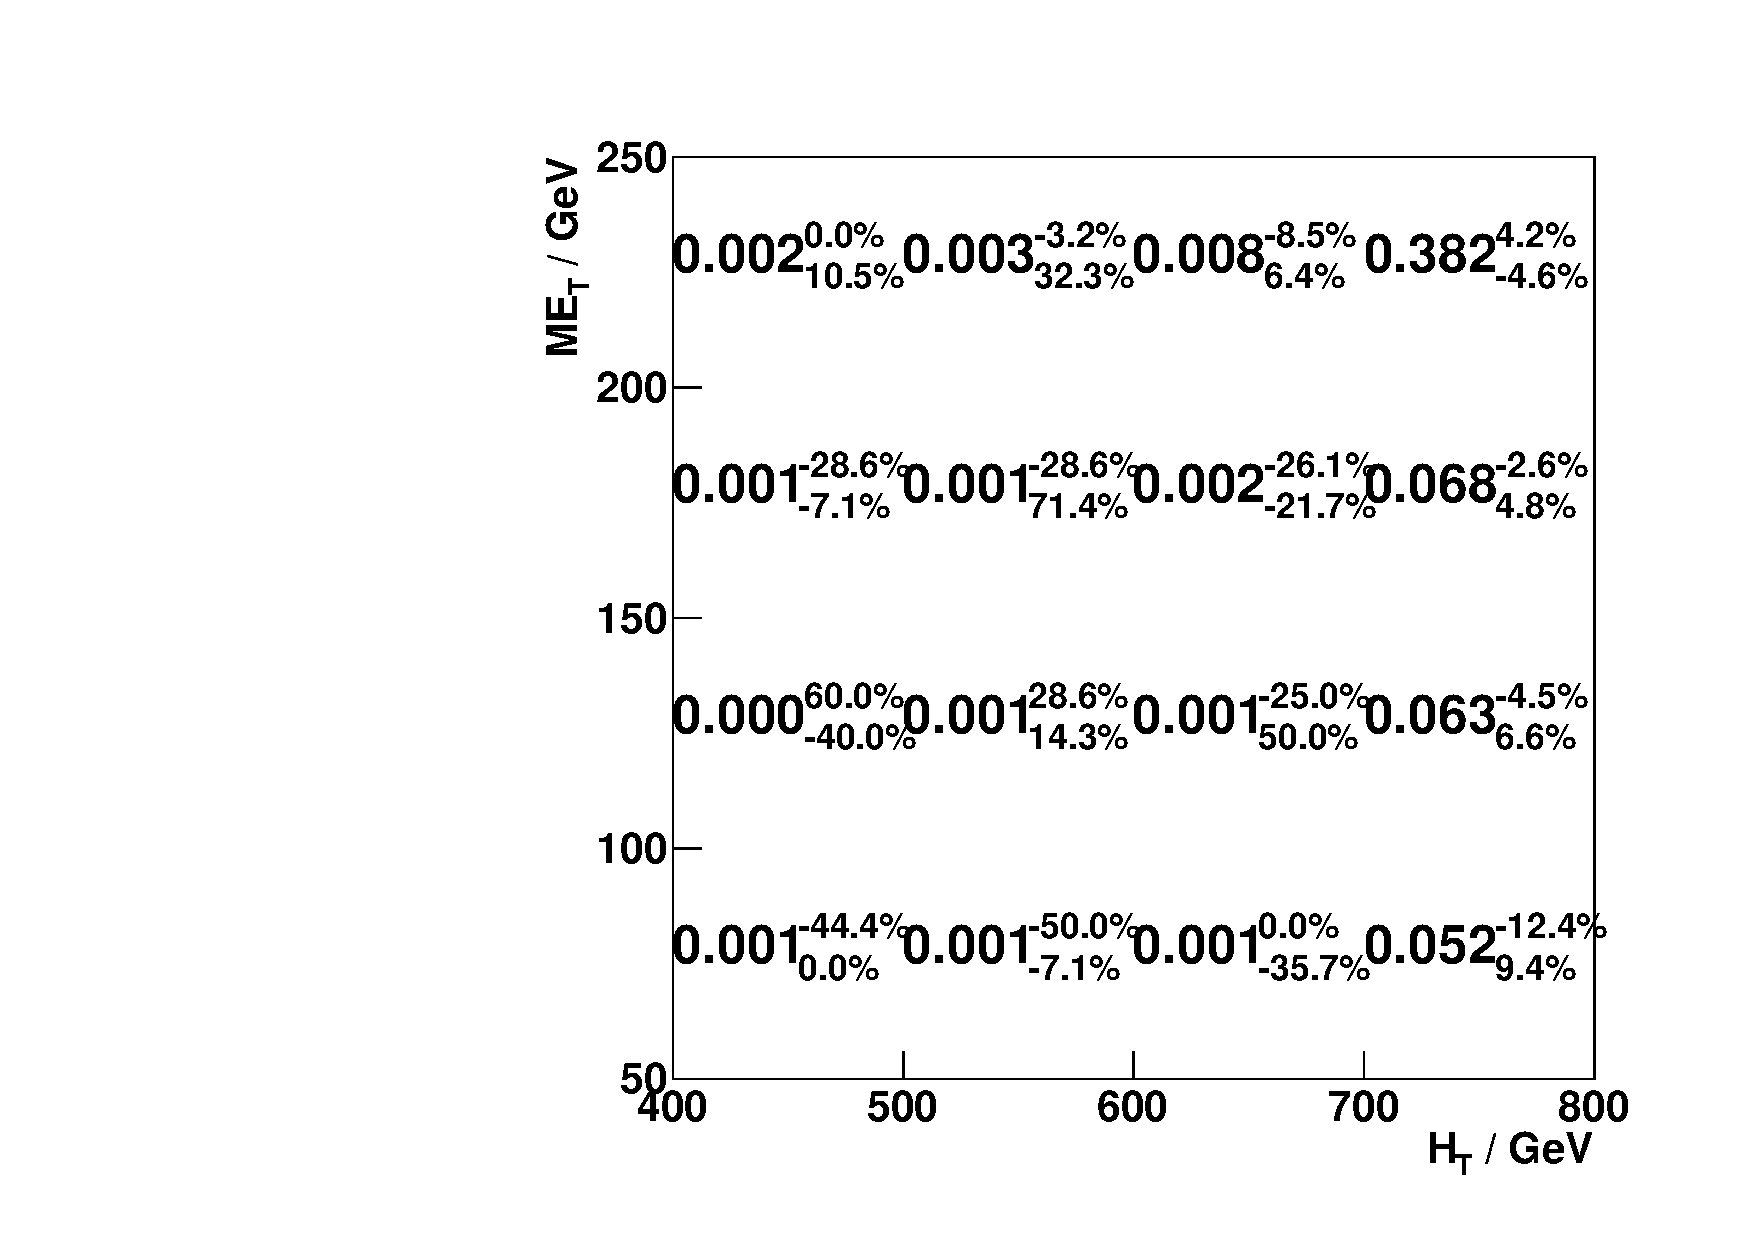
\includegraphics[width=0.7\textwidth]{SUSY_150_1040_1200_JES.pdf}
\end{center}
\caption{The percentage change in the signal efficiency when the jet energy
scale is varied by $\pm1\sigma$, where $\sigma$ is the jet energy scale
uncertainty.}
\label{fig:JES_Numbers}
\end{figure}

\section{Jet Energy Resolution}

The jet $\pT$ resolution is determined using two different methods: 

\begin{itemize}
\item {\bf Di-jet asymmetry:} This method uses balanced di-jet events which are 
abundant in data and considers $\pT$ conservation. An asymmetry variable is 
constructed from the $\pT$ of the two jets:
\begin{equation}
A = \frac{\pT^{1} - \pT^{2}}{\pT^{1} + \pT^{2}}
\end{equation}
The variance of the asymmetry variable can be expressed as:
\begin{equation}
\sigma_{A}^{2} = \left(\frac{\partial A}{\partial
\pT^{1}}\right)^{2}\sigma_{\pT^{1}}^{2} + \left(\frac{\partial A}{\partial
\pT^{2}}\right)^{2}\sigma_{\pT^{2}}^{2}
\end{equation}
For jets which lie in the same $\eta$ bin and the same $\pT$ bin, the $\pT$'s
are the same and the reslutions are the same so there is an expression for the
fractional $\pT$ resolution in terms of the variance in the asymmetry.
\begin{equation}
\frac{\sigma_{\pT}}{\pT} = \sqrt{2}\sigma_{A}
\end{equation}  
The asymmetry and the variance in the asymmetry are quantities that can be 
measured in data.
\item {\bf $\gamma$/Z+jet balance:} This method uses $\gamma$+jet or Z+jet
events from data and uses the $\gamma$ or Z as a well measured reference object
to which the jet $\pT$ can be compared. In balanced events the $\gamma$/Z has 
the same $\pT$ as the jet. The ratio, R, of the jet $\pT$ relative to the 
$\gamma$/Z $\pT$ in bins of $\gamma$/Z $\pT$ gives the jet $\pT$ resolution. 
\begin{equation}
R = \frac{\pT^{jet}}{\pT^{\gamma/Z}}
\end{equation}
\end{itemize}

\begin{figure}
\begin{center}
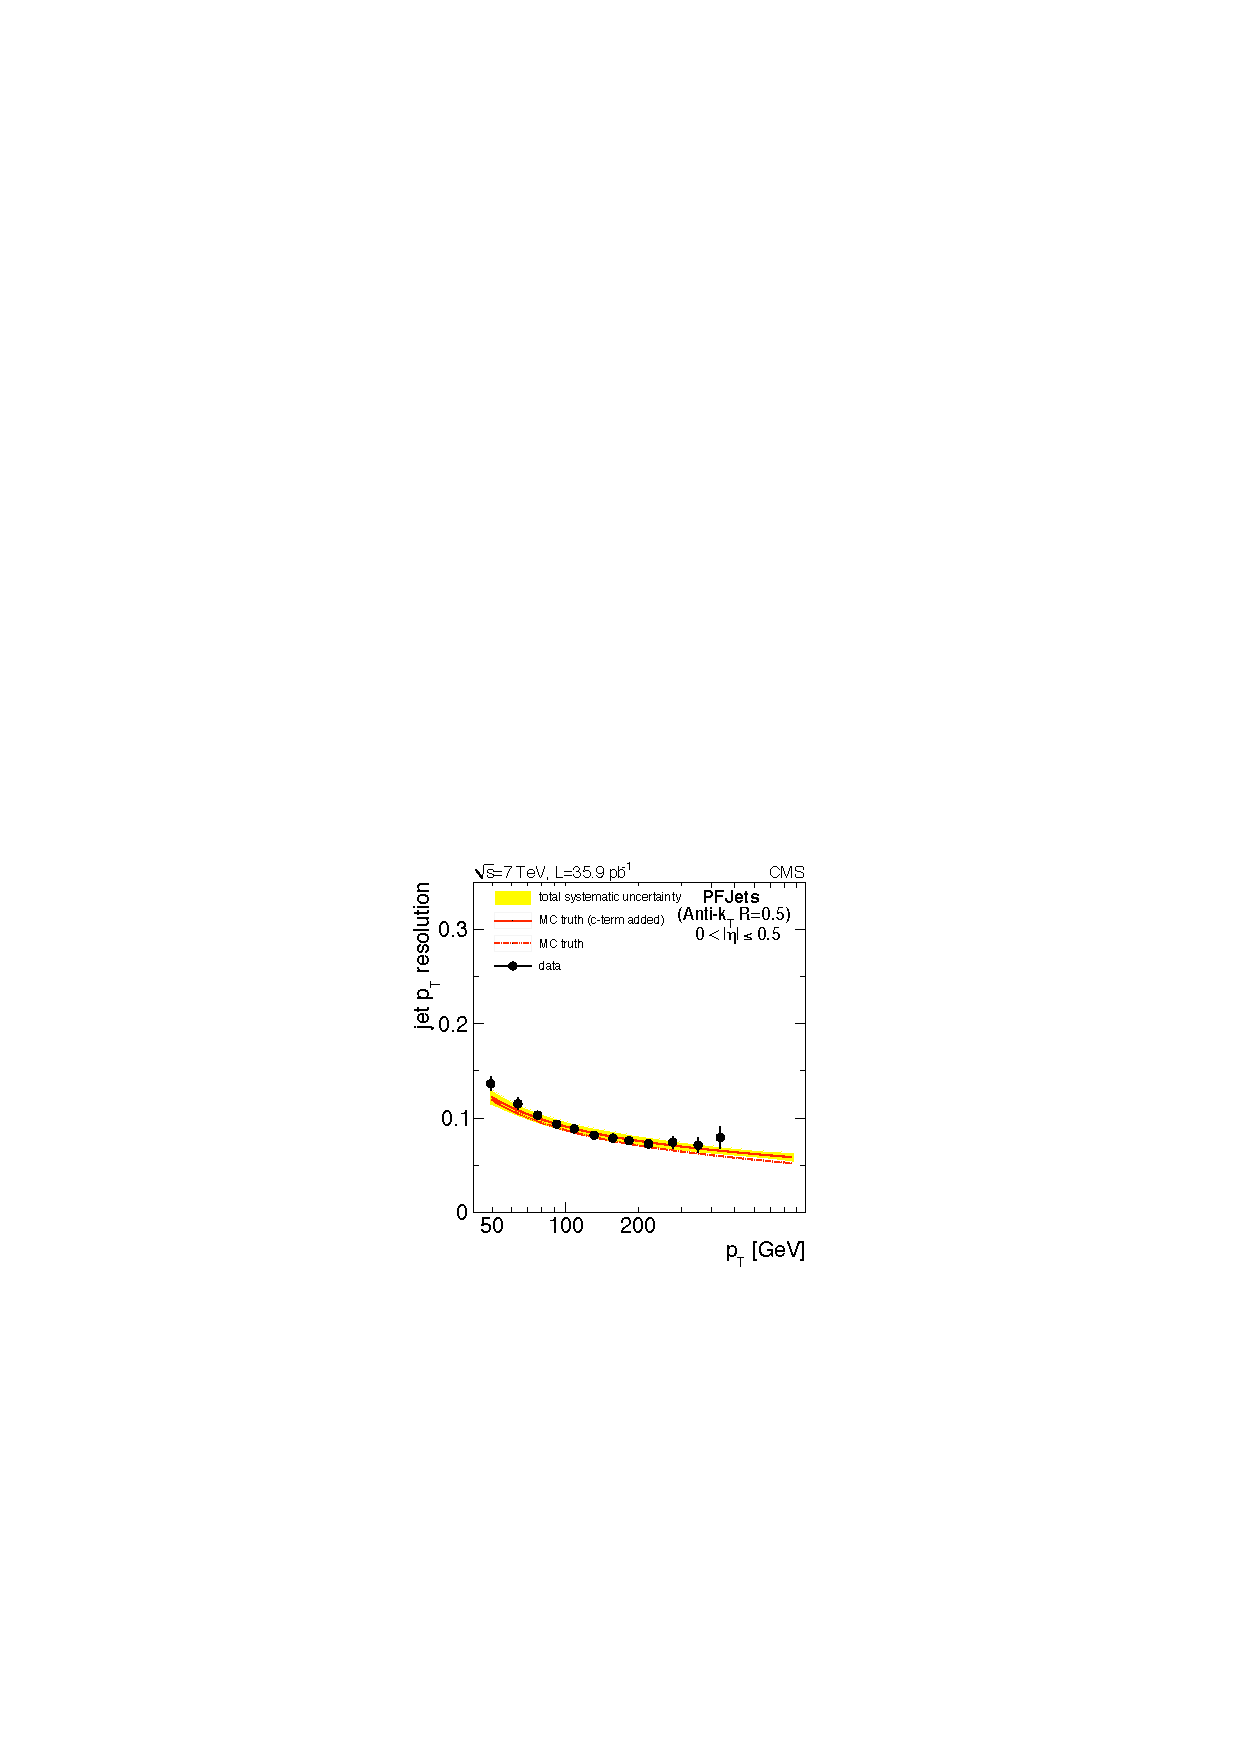
\includegraphics[width=0.7\textwidth]{Jet_pT_Resolution.pdf}
\end{center}
\caption{The jet energy resolution measured from data for jets with $|\eta| <
0.5$ (black points) compared to MC (red line). The yellow band gives the
systematic uncertainty. Reproduced from \cite{jec}.}
\label{fig:Jet_pT_Resolution}
\end{figure}

Further details on the jet $\pT$ resolution measurement and determination of the
associated uncertainty can be found in \cite{jec}. The jet $\pT$ resolution as a
function of jet $\pT$ and for $|\eta| < 0.5$ is shown in Figure
\ref{fig:Jet_pT_Resolution}. The figure also shows that MC agrees well with the
data as far as jet enrgy resolution is concerned. For the SUSY events the 
``true'' jet energy comes from the generator level in the MC. The jet energy 
resolution is determined by comparing the reconstructed jet energy with the 
generator level jet energy. This gives a jet $\pT$ resolution similar to that 
measured in \cite{jec}. \\

\begin{figure}
\begin{center}
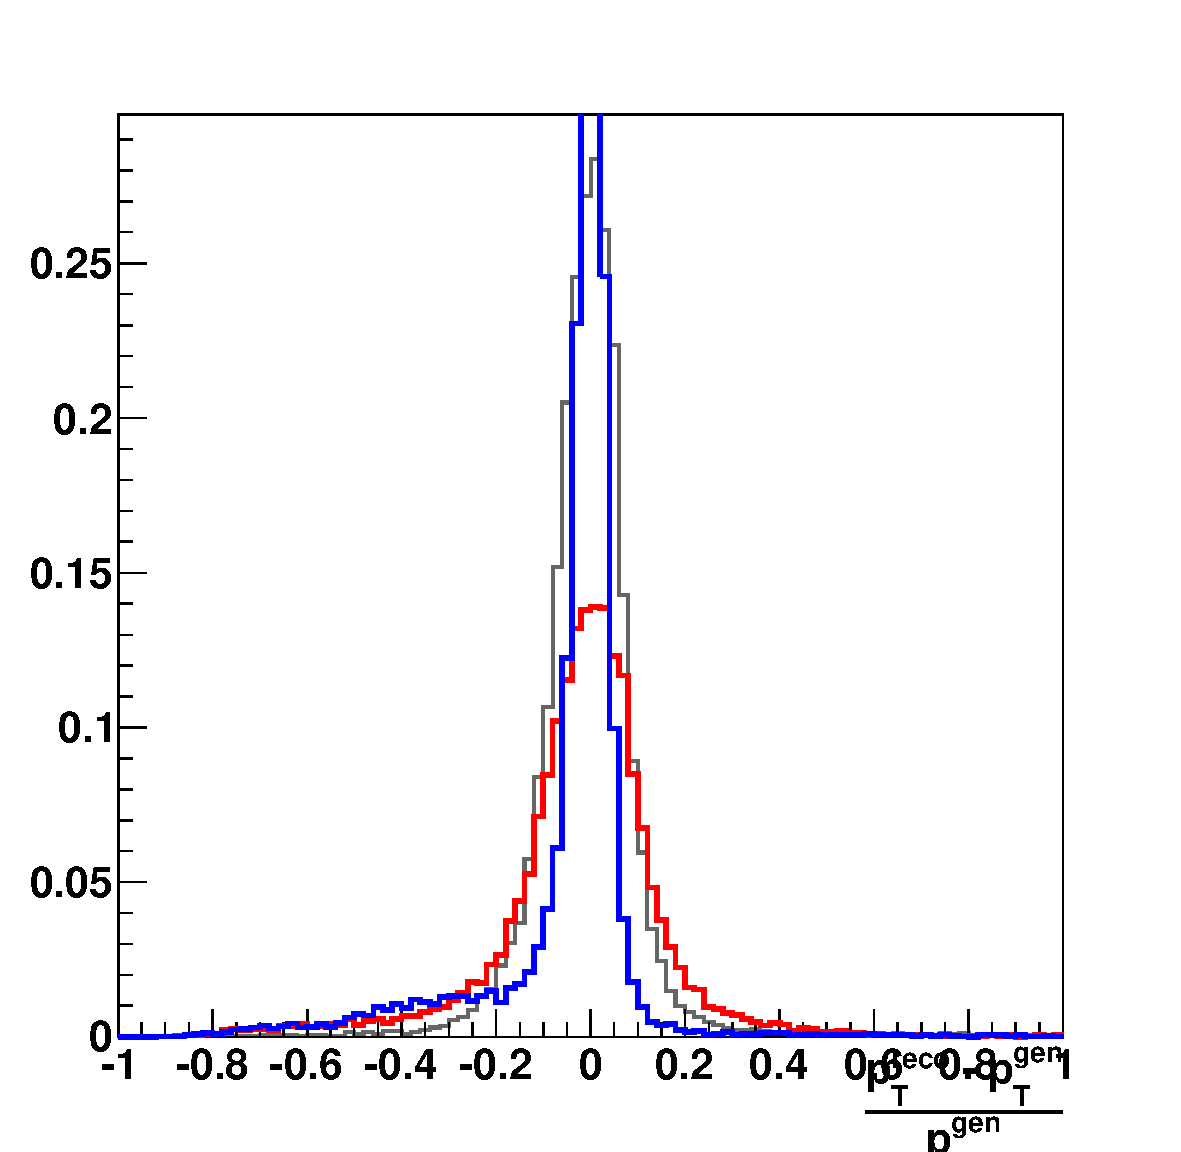
\includegraphics[width=0.7\textwidth]{Resolution.pdf}
\end{center}
\caption{The jet $\pT$ resolution compared to generator level jets (grey) and
the same distribution after an upward (red) and downward (blue) 
variation of 50\% in the jet $\pT$ resolution.}
\label{fig:Resolution}
\end{figure}

The resolution is varied upward and downward by 50\%, which correspond to the 
uncertainty on the forward jets but is conservative for the central jets. The
variation in resolution is made by changing $\frac{\pT^{reco} -
\pT^{gen}}{\pT^{gen}}$ by 50\% for each jet. Figure \ref{fig:Resolution}
shows the jet energy reolution with an upward and a downward variation. \\

\begin{figure}
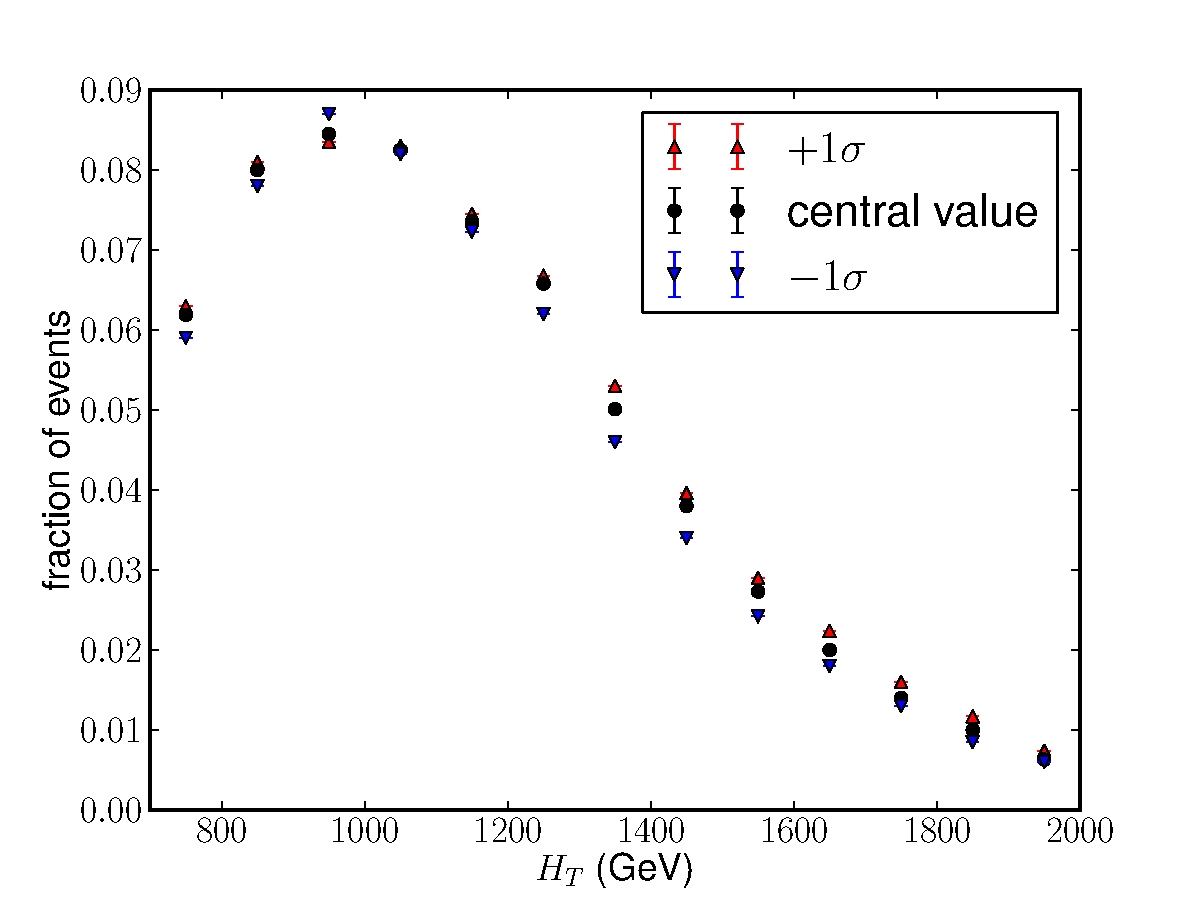
\includegraphics[width=0.5\textwidth]{JER_HT.pdf}
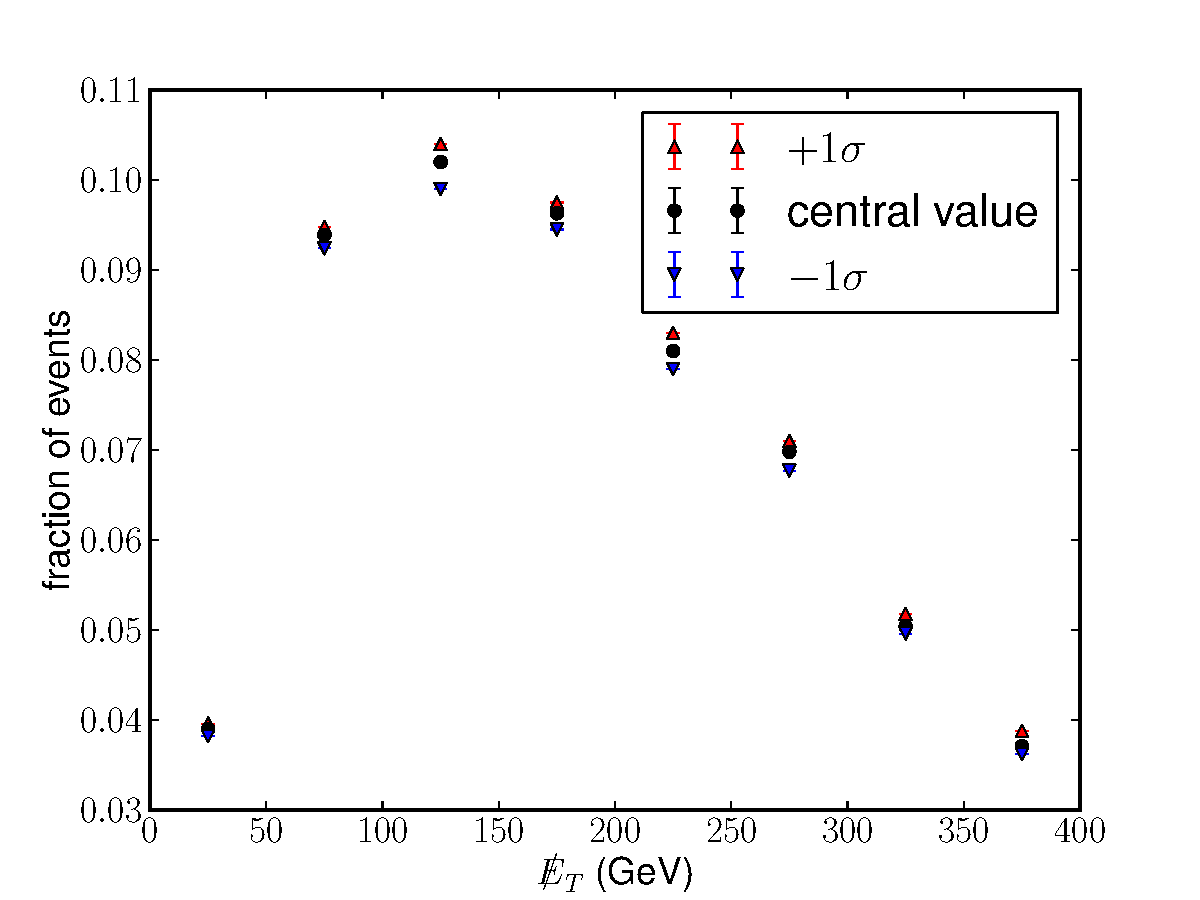
\includegraphics[width=0.5\textwidth]{JER_MET.pdf}
\caption{The effect of an upward (red) and a downward (blue) variation
of the jet $\pT$ resolution on the $\HT$ and $\MET$ distributions.}
\label{fig:JER}
\end{figure}

Figure \ref{fig:JER} shows the effect of the variation in resolution on the
$\HT$ and $\MET$ distributions. The important result is how the variation in jet
energy scale affects the signal efficiency in each ($\HT$, $\MET$) bin. Figure 
\ref{fig:JES_Numbers} shows these numbers. The jet energy scale uncertainties 
are correlated across all ($\HT$,$\MET$) bins.

\begin{figure}
\begin{center}
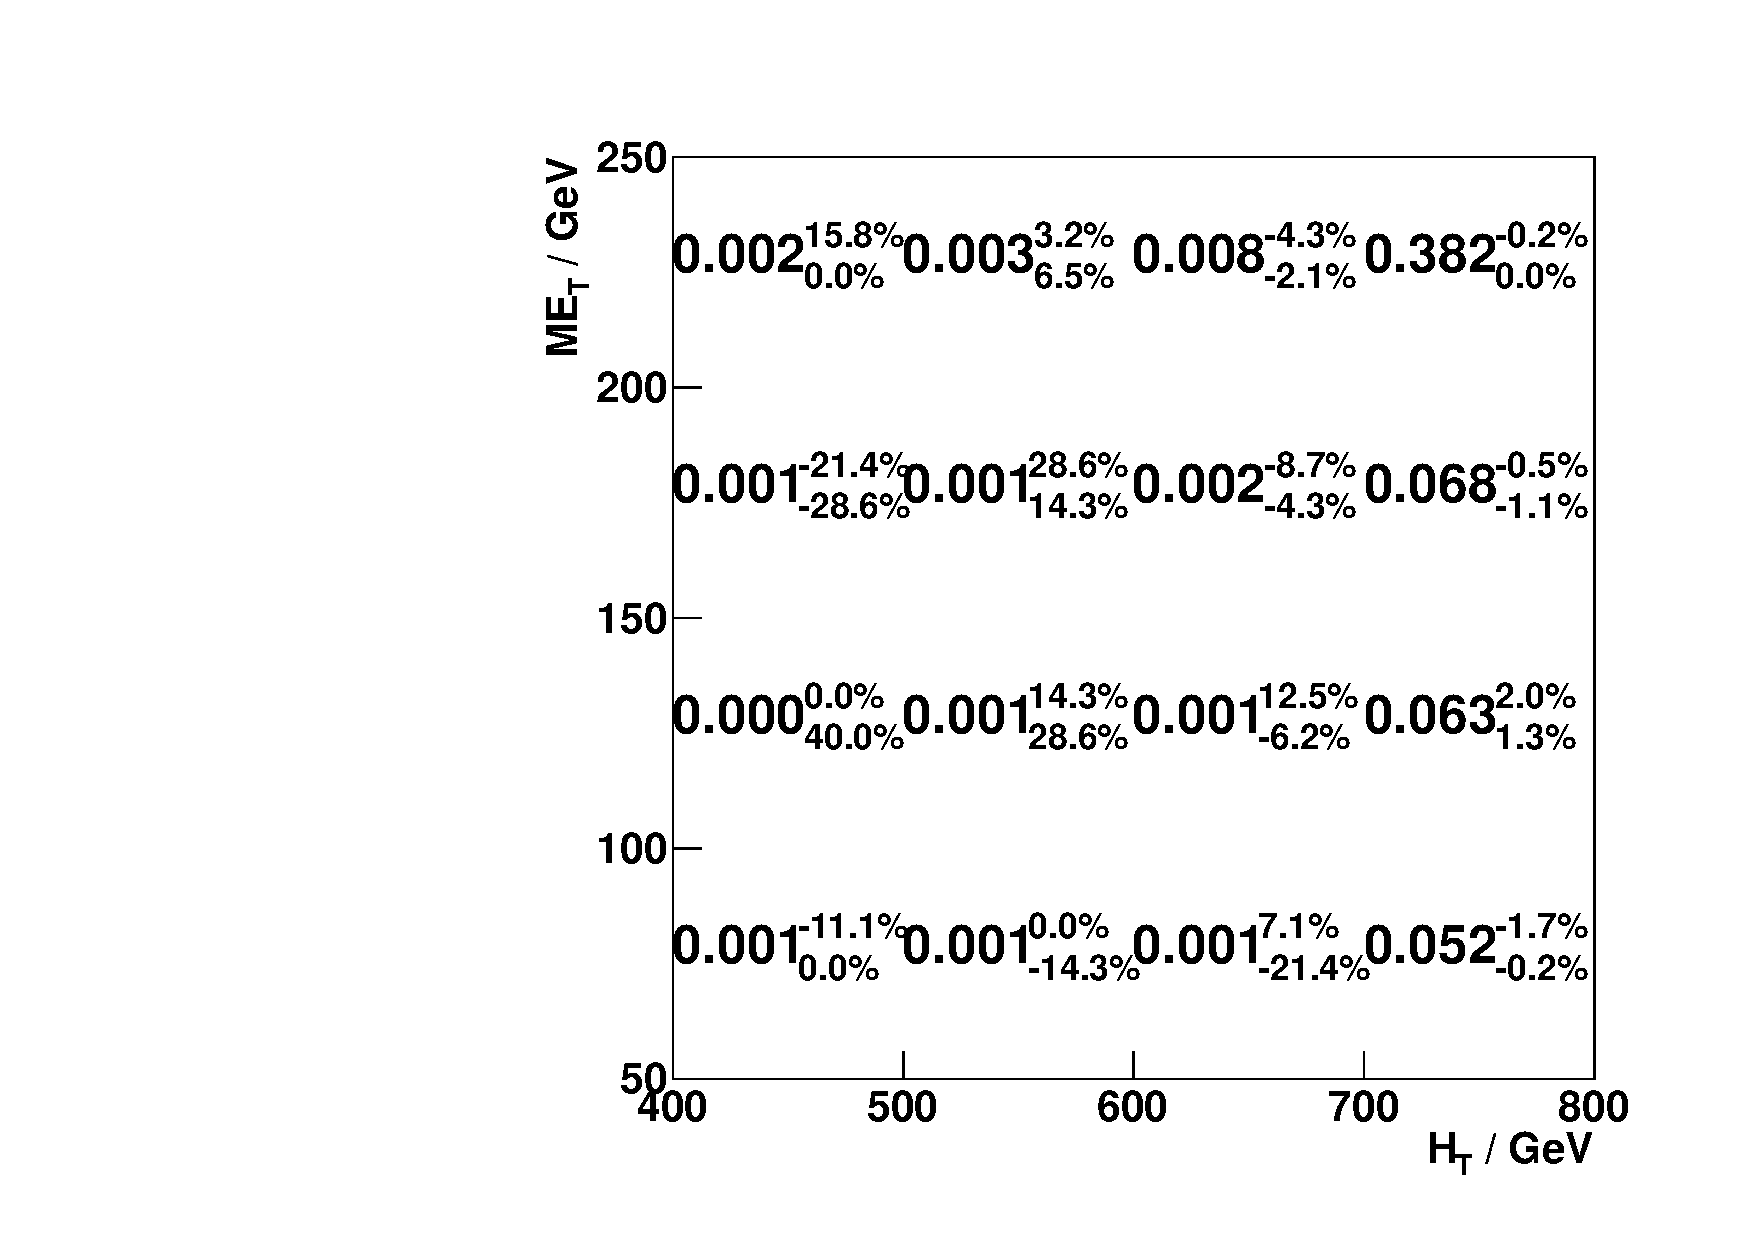
\includegraphics[width=0.7\textwidth]{SUSY_150_1040_1200_JER.pdf}
\end{center}
\caption{The percentage change in the signal efficiency when the jet $\pT$
resolution is varied by $\pm1\sigma$, where $\sigma$ is the jet $\pT$ resolution 
uncertainty.}
\label{fig:JER_Numbers}
\end{figure}

\section{Pile-up}

Pile-up is where there are multiple interations per bunch crossing. 
%Some of the
%effects of pile-up are avoided by requiring that the two jets and the photon
%come from the same primary vertex as they must in the SUSY event hypothesis. 
Pile-up affects the number of signal events in several ways:

\begin{itemize}
\item The $\HT$ increases due to jets and underlying event activity from other 
interactions in the same bunch crossing.
\item The $\MET$ distribution is broadened by the introduction of more jets and
underlying event activity.
\item The photon isolation efficiency is reduced since there is more 
surrounding activity which can populate the isolation cone.
\end{itemize}

Most of the pile-up events will be soft QCD with low $\pT$ jets approximately 
parallel to the beam-line. These do not have a huge effect on the $\HT$ since 
the $\HT$ is a sum of high $\pT$ jets. The effect of pile-up on the $\HT$ is 
evaluated by looking at the HT distribution in MC QCD events with and without 
pile-up. A shift of $7.0\pm0.8$ is applied to the no pile-up $\HT$ distribution 
to match the pile-up $\HT$ distribution (Figure \ref{fig:meanht_vs_htshift}). 
Figure \ref{fig:puHT} shows the $\HT$ distribution with a $\pm 1$ sigma 
variation in the shift. \\

\begin{figure}
\begin{center}
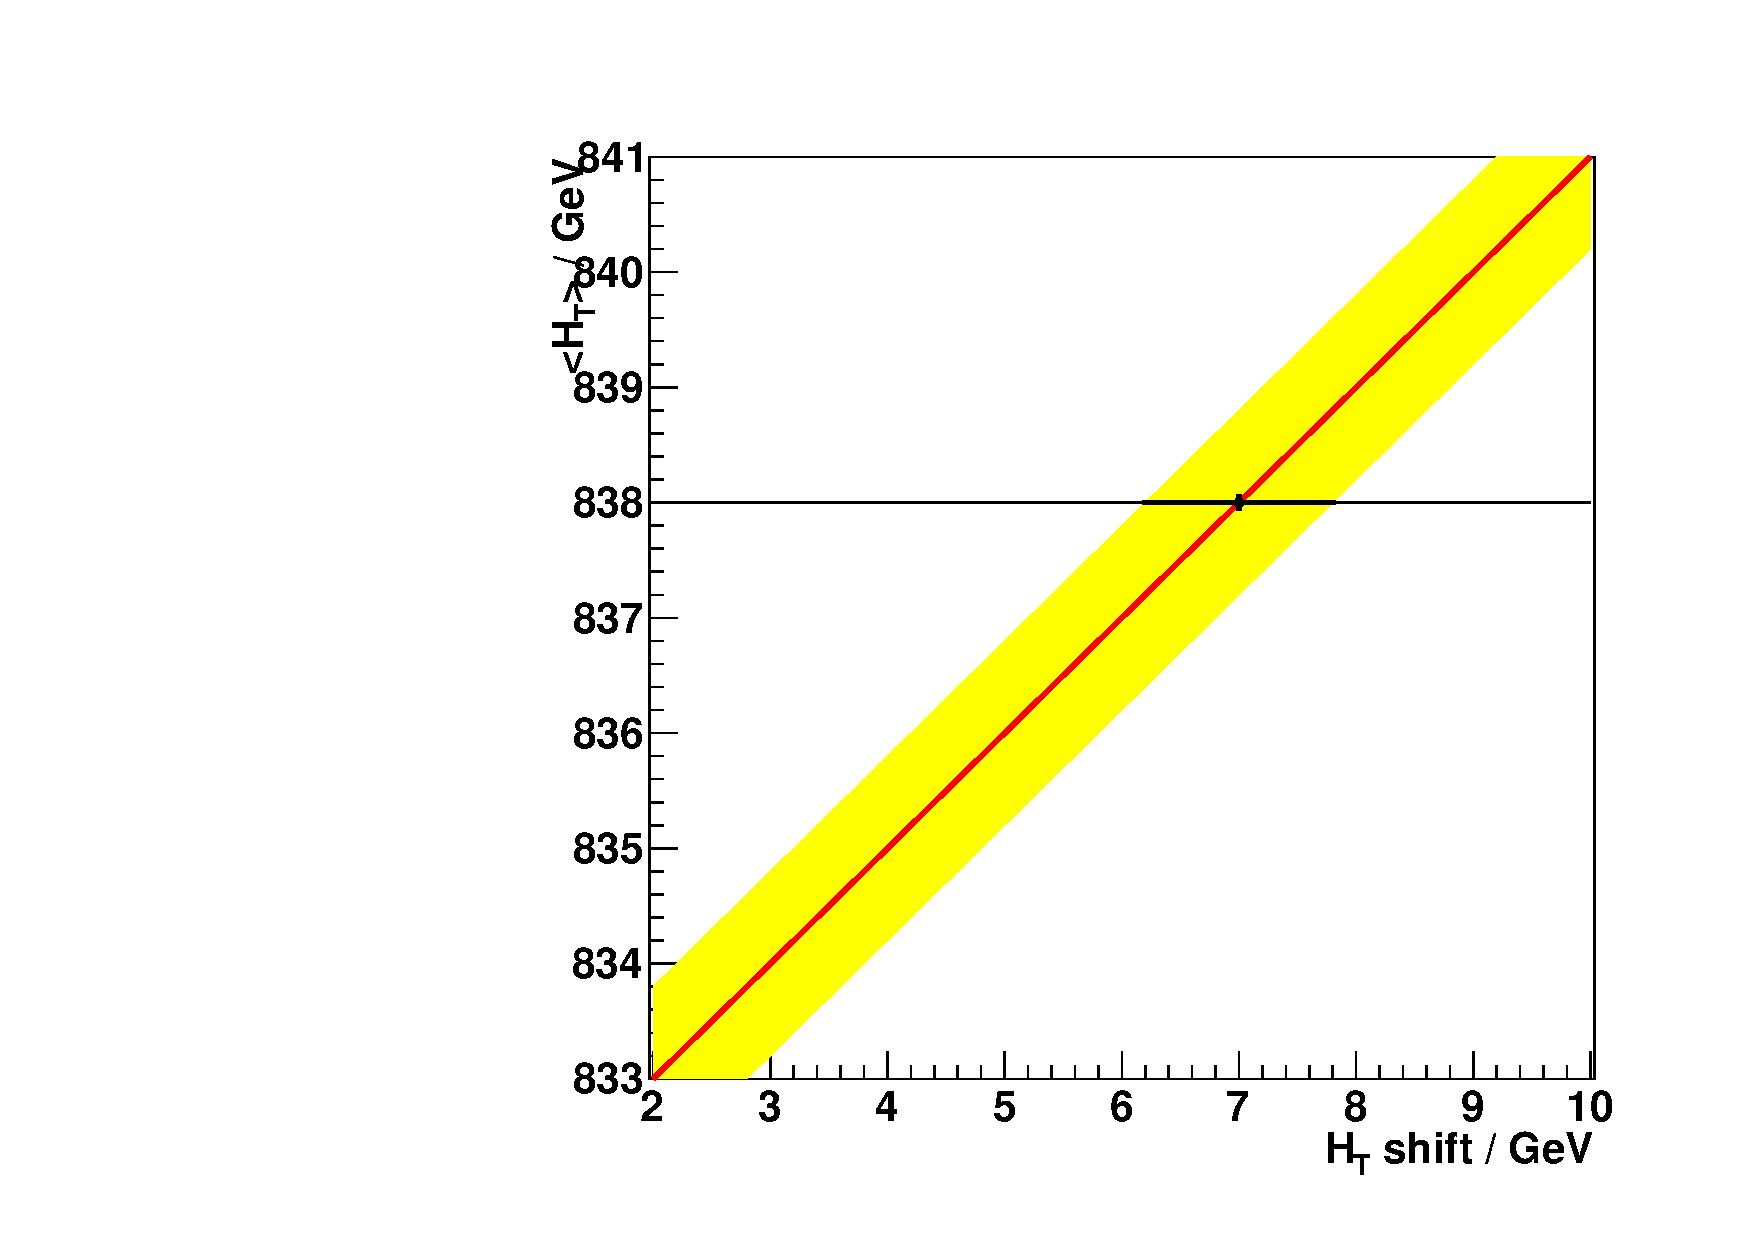
\includegraphics[width=0.7\textwidth]{meanht_vs_htshift.pdf}
\end{center}
\caption{The mean $\HT$ as a function of $\HT$ shift (red) with one sigma band 
(yellow) in QCD events with a similar $\HT$ to the signal. The mean $\HT$ with 
pile-up is shown in black.}
\label{fig:meanht_vs_htshift}
\end{figure}

\begin{figure}
\begin{center}
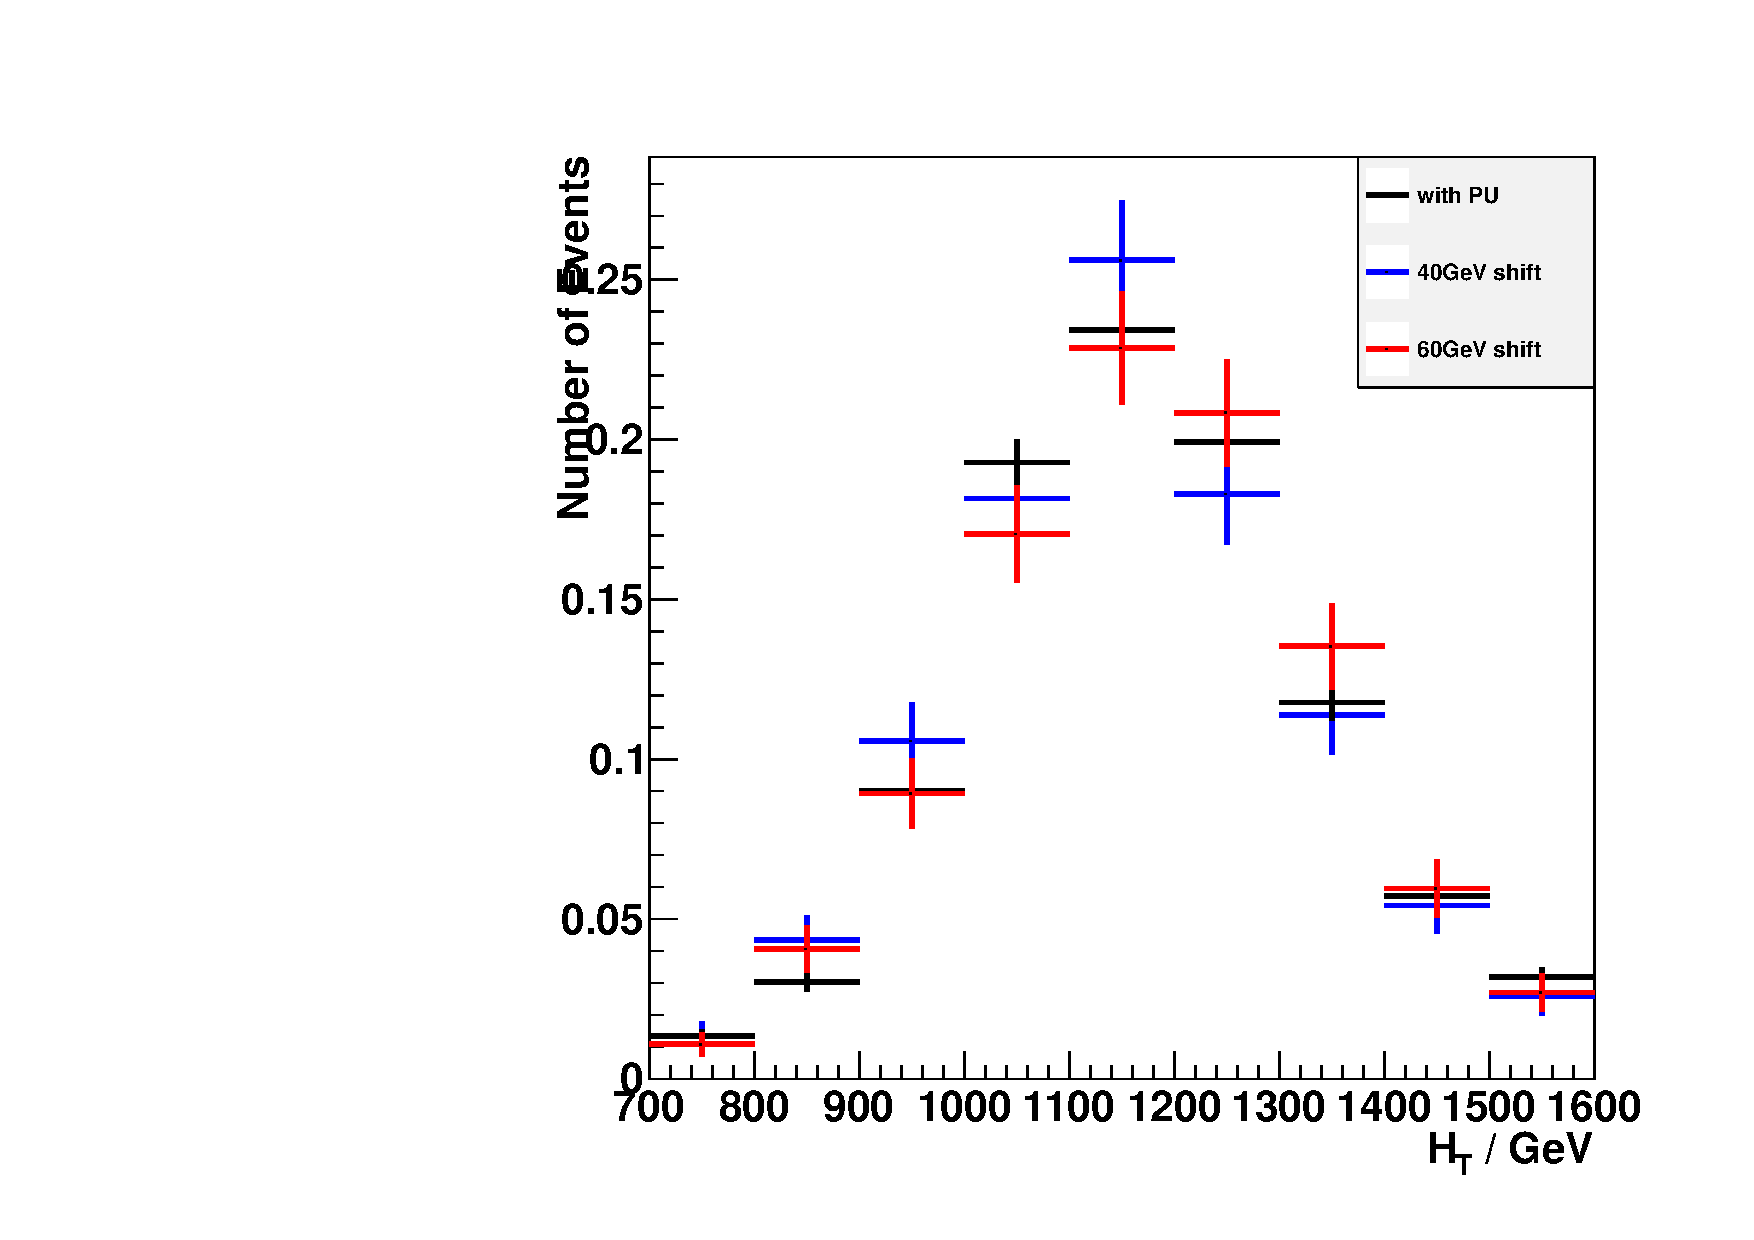
\includegraphics[width=0.7\textwidth]{puHT.pdf}
\end{center}
\caption{The correction to the $\HT$ distribution to account for pile-up. The
$\pm 1$ sigma variations are shown in red and blue respectively.}
\label{fig:puHT}
\end{figure}

\begin{figure}
\begin{center}
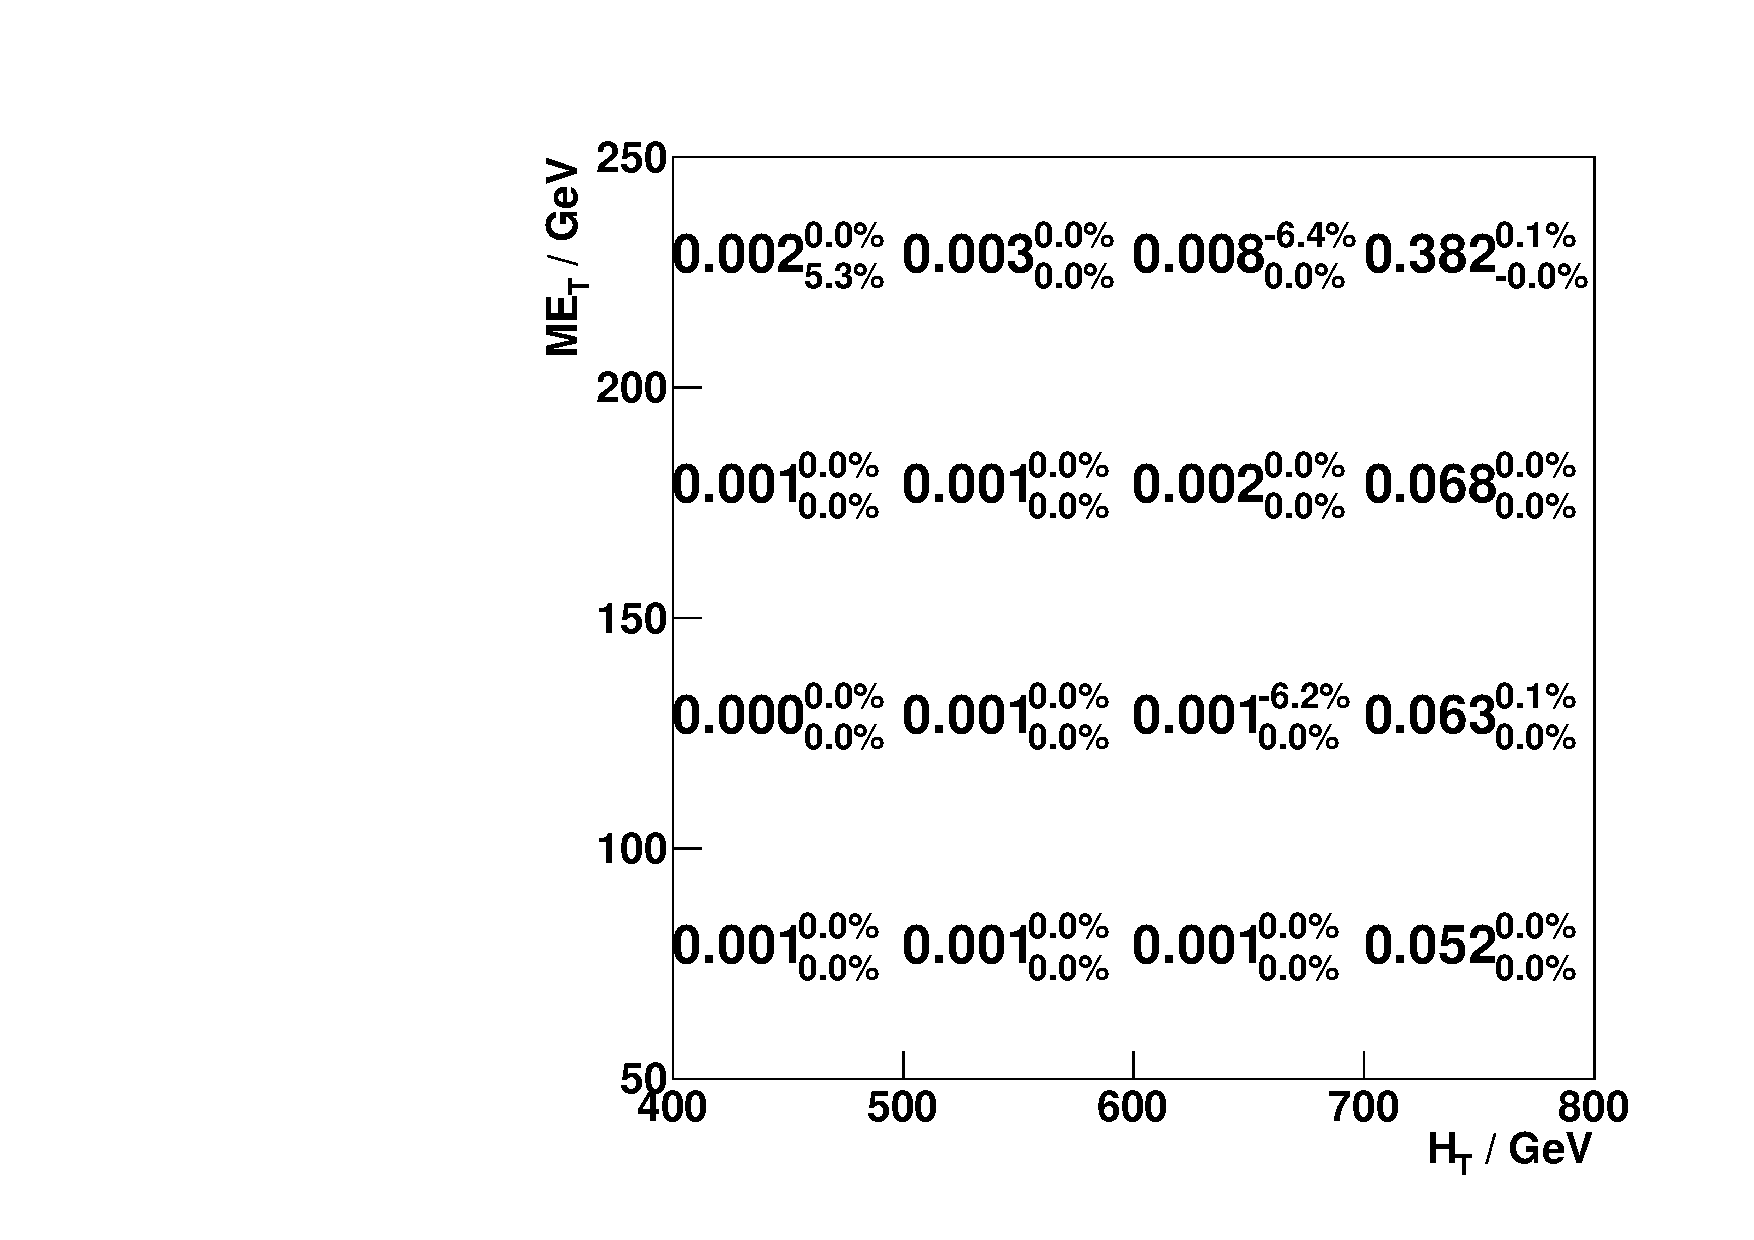
\includegraphics[width=0.7\textwidth]{SUSY_150_1040_1200_htPU.pdf}
\end{center}
\caption{The percentage change in the signal efficiency when the $H_{T}$ shift
to account for pile-up is varied within its uncertainty.} 
\label{fig:puHT_Numbers}
\end{figure}

The $\MET$ distribution is broadened by the introduction of more jets from other
interactions in the same bunch crossing. The pile-up events will mostly be low
$\HT$ and balanced so will have only a little effect on the $\MET$. The $\MET$
distribution is smeared to account for pile-up. To determine the amount of
smearing necessary a QCD sample with similar $\HT$ and no pile-up is smeared
until the shape agrees with the $\MET$ distribution with pile-up. Figure 
\ref{fig:meanmet_vs_metsmearing} shows the average $\MET$ in QCD events without 
pile-up as a function of the $\MET$ smearing. From the plot a $\MET$ smearing of 
$2.9\pm0.8\%$ is applied to account for pile-up. Figure \ref{fig:puMET} shows the 
$\MET$ distribution with a $\pm 1$ sigma variation in the shift. \\

\begin{figure}
\begin{center}
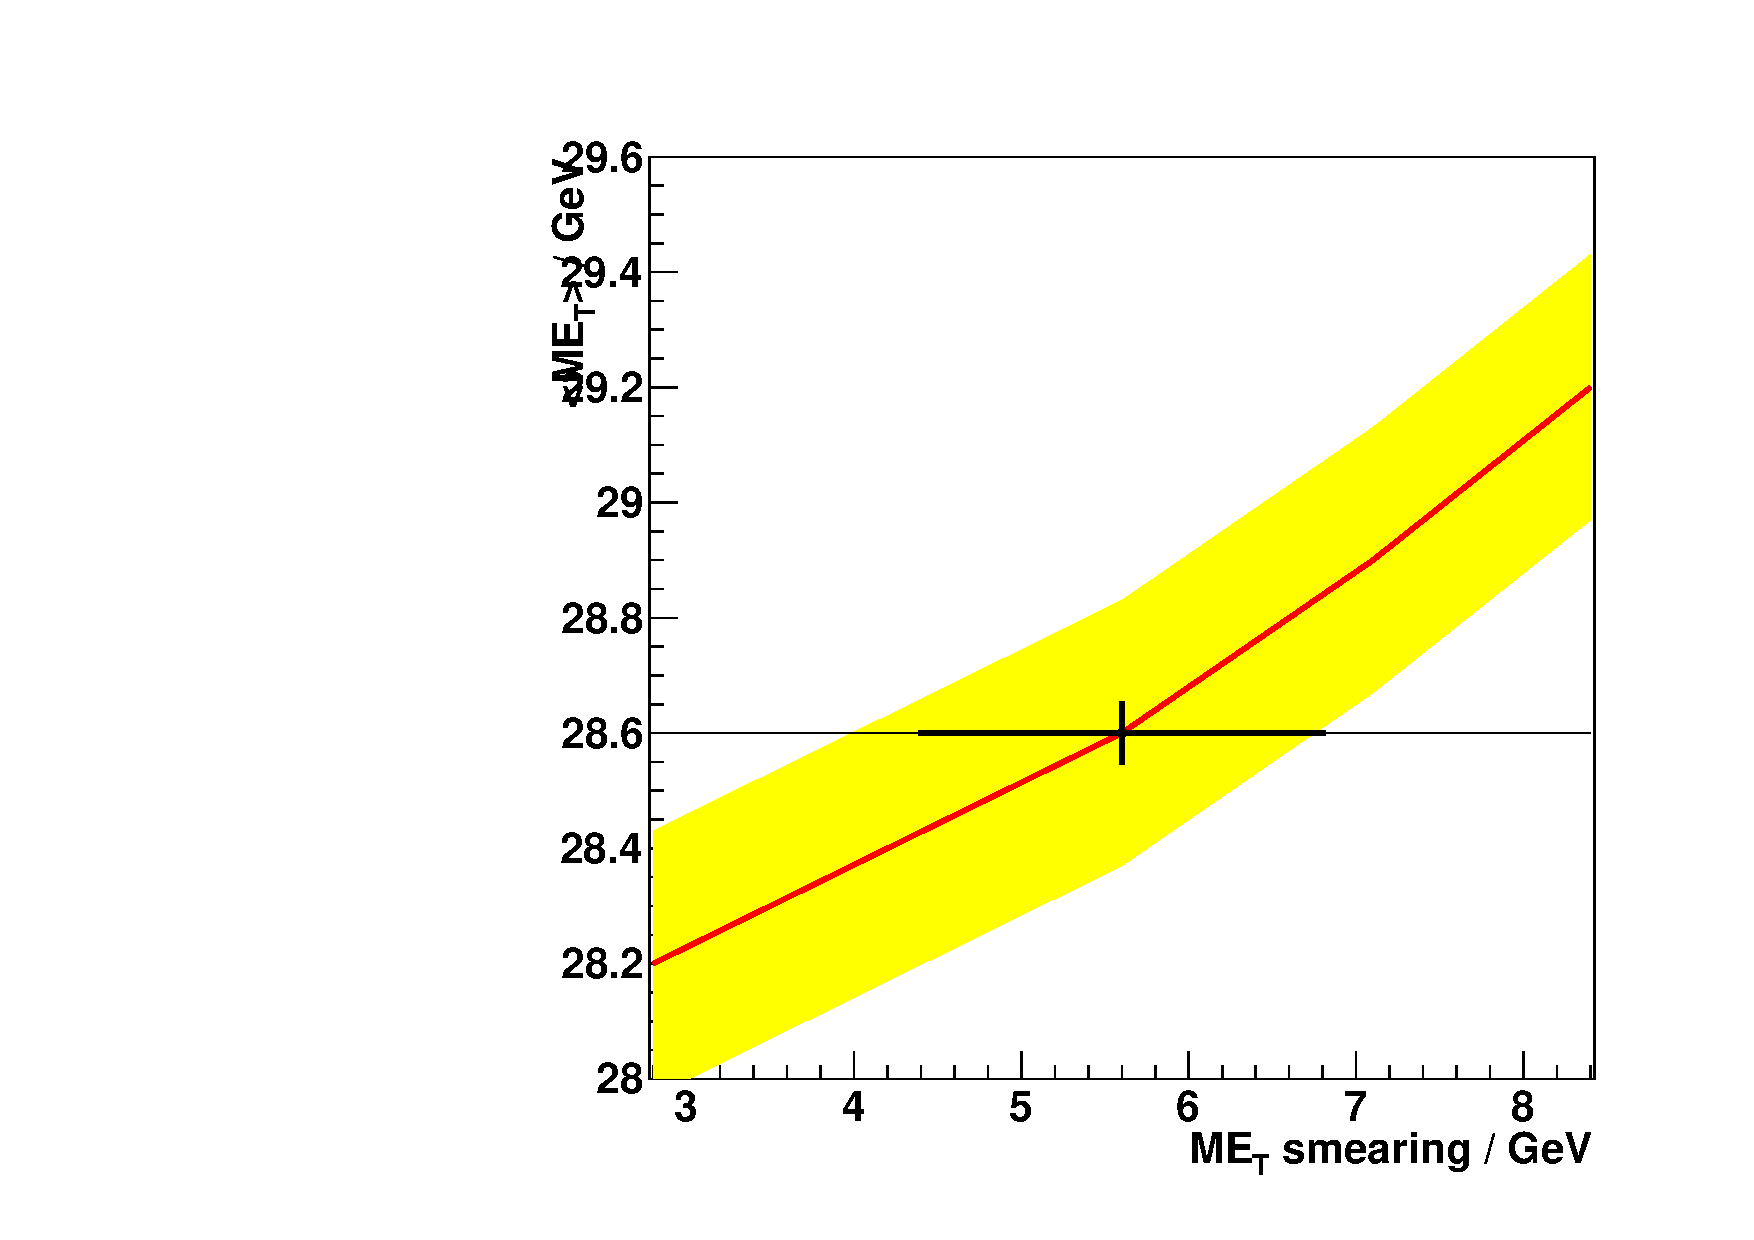
\includegraphics[width=0.7\textwidth]{meanmet_vs_metsmearing.pdf}
\end{center}
\caption{The mean $\MET$ as a function of $\MET$ smearing (red) with one sigma
band (yellow) in QCD events with a similar $\HT$ to the signal. The mean $\MET$ 
with pile-up is shown in black.}
\label{fig:meanmet_vs_metsmearing}
\end{figure}

\begin{figure}
\begin{center}
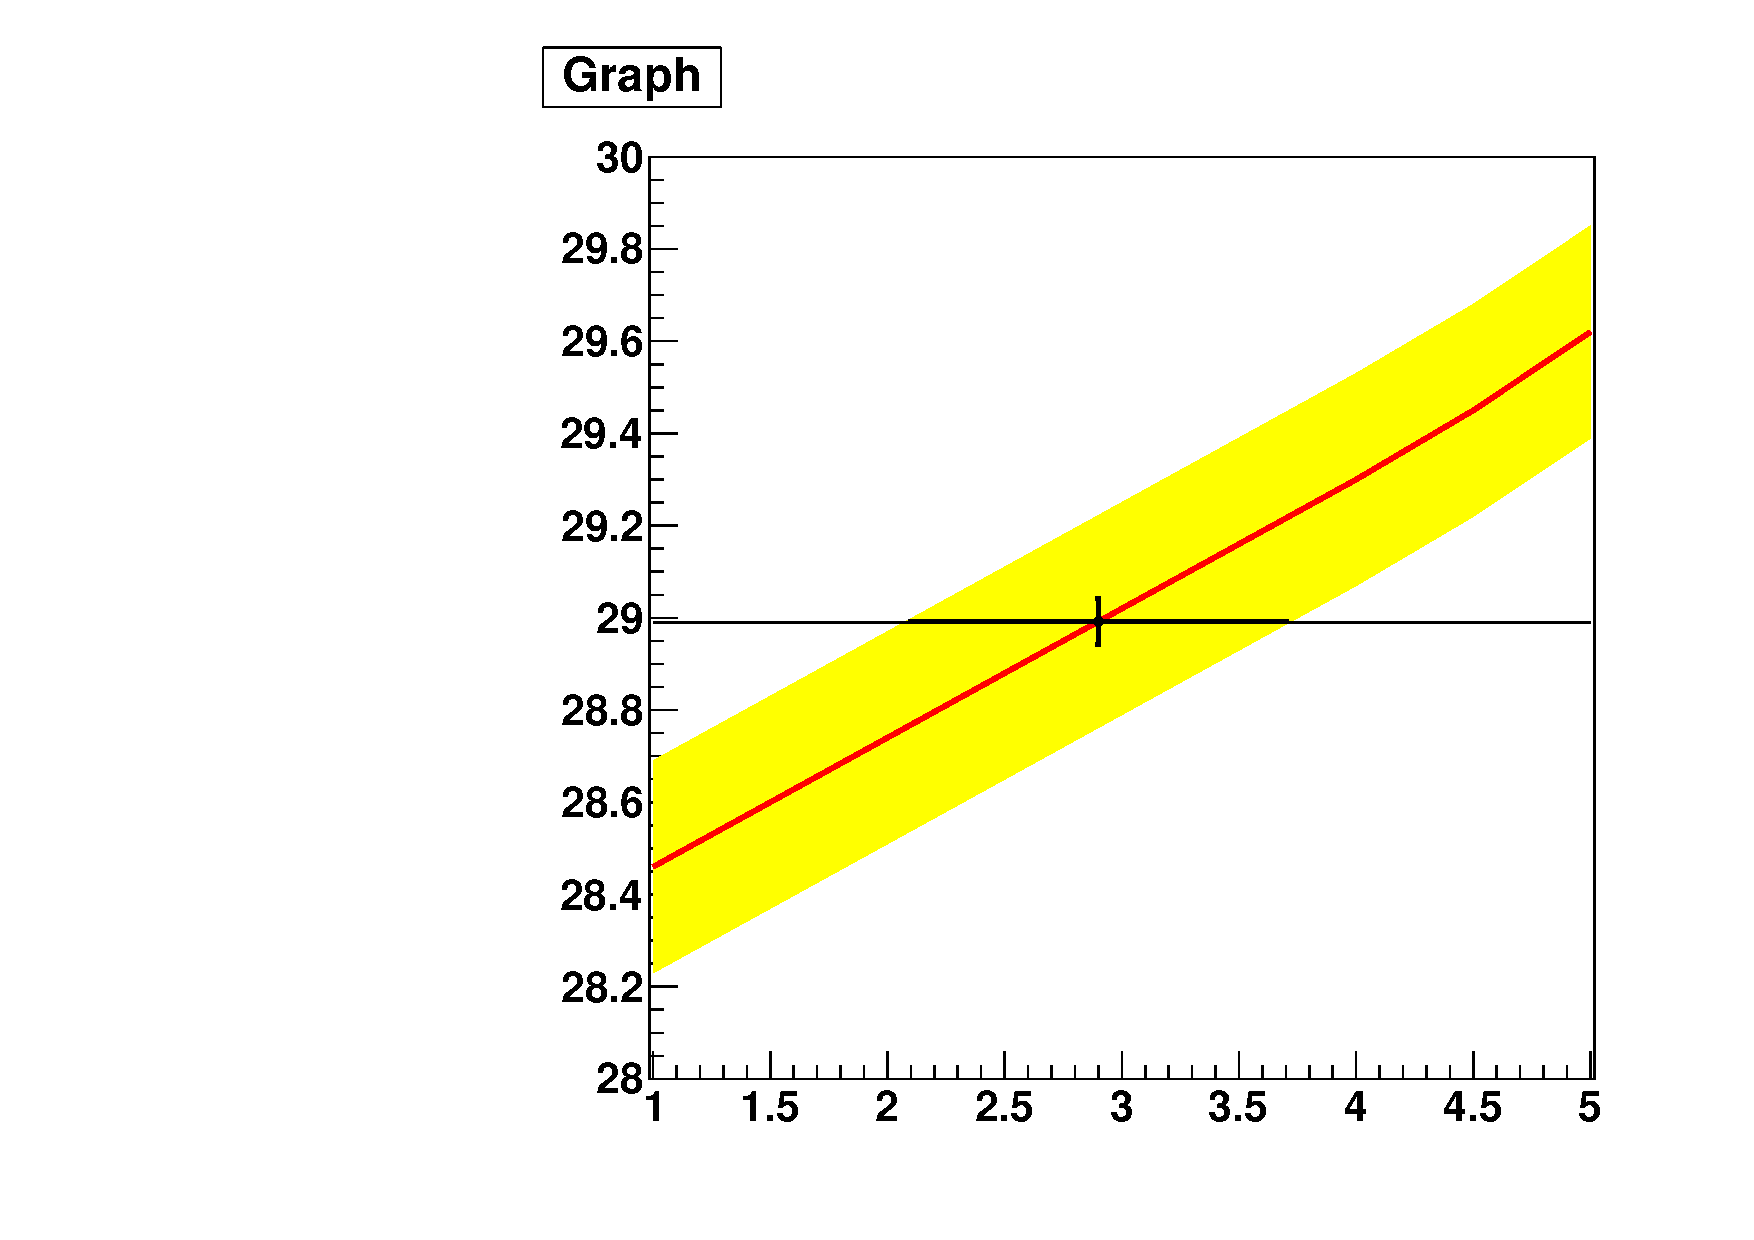
\includegraphics[width=0.7\textwidth]{puMET.pdf}
\end{center}
\caption{The correction to the $\MET$ distribution to account for pile-up. The
$\pm 1$ sigma variations are shown in red and blue respectively.}
\label{fig:puMET}
\end{figure}

\begin{figure}
\begin{center}
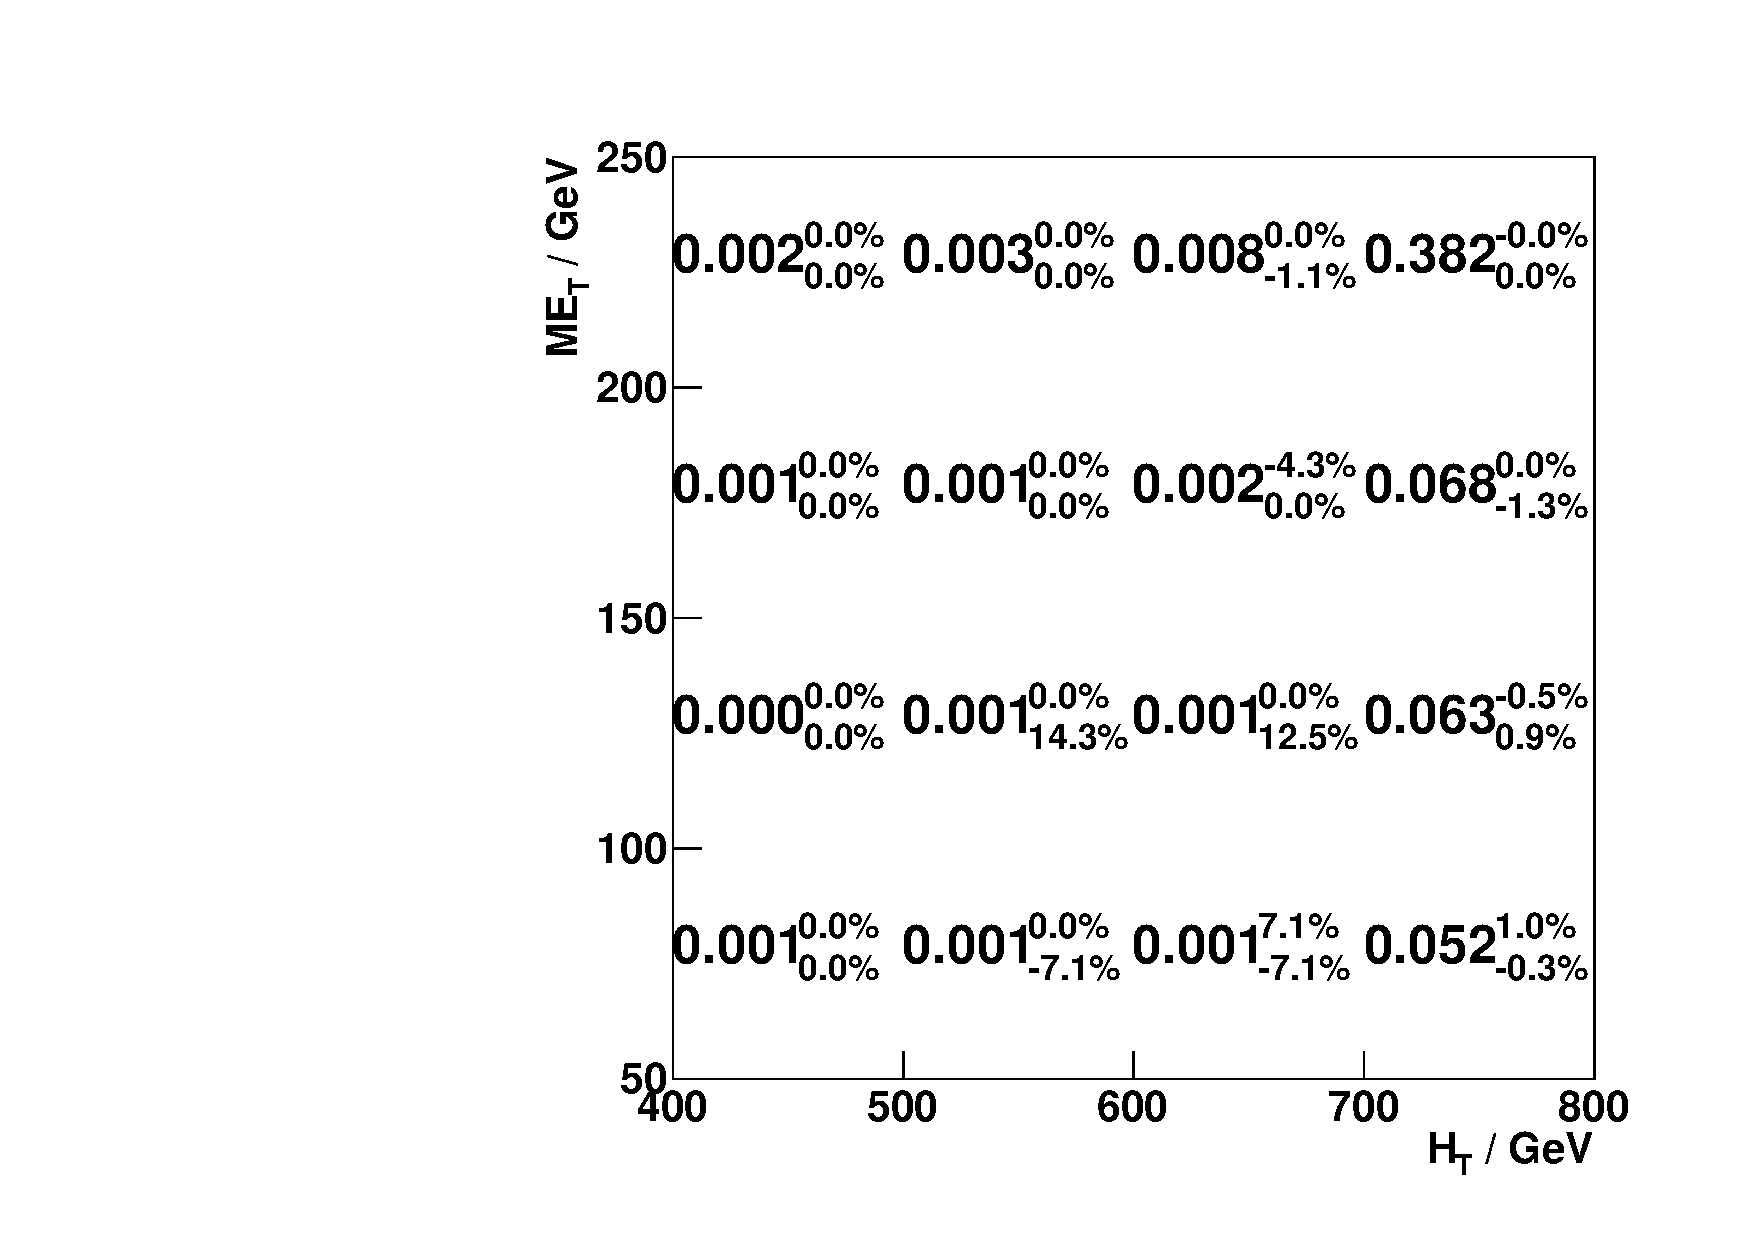
\includegraphics[width=0.7\textwidth]{SUSY_150_1040_1200_metPU.pdf}
\end{center}
\caption{The percentage change in the signal efficiency when the $ME_{T}$
smearing to account for pile-up is varied within its uncertainty.} 
\label{fig:puMET_Numbers}
\end{figure}

The photon isolation efficiency is particularly affected by pile-up because
activity from other events in the same bunch crossing can populate the isolation
cone. To quantify this effect QCD MC events with a similar $\HT$ were used to
determine the photon efficiency in MC as a function of the number of primary
vertices. Figure \ref{fig:Efficiency_vs_nVertices} shows the relative efficiency
as a function of the number of primary vertices. Taking the distribution of 
number of primary vertices from data, the efficiency expected under pile-up can 
be calculated. This method assumes that SUSY photons have a similar behaviour 
under pile-up to QCD photons. This assumption is reasonable beacause the pile-up 
affects mainly the isolation through extra surrounding activity which is a 
property of the event rather than the photon. This method also relies on MC 
modelling the photon efficiency in pile-up well. This can be checked by looking 
at Zee events in data. The efficiency requires only a small correction between 
data and MC which is relatively stable with respect to pile-up (Figure 
\ref{fig:EffCorr_vs_nPV}). The efficiency correction due to pile-up is found to 
be $0.83\pm0.01(stat.)\pm0.01(syst.)$. \\

\begin{figure}
\begin{center}
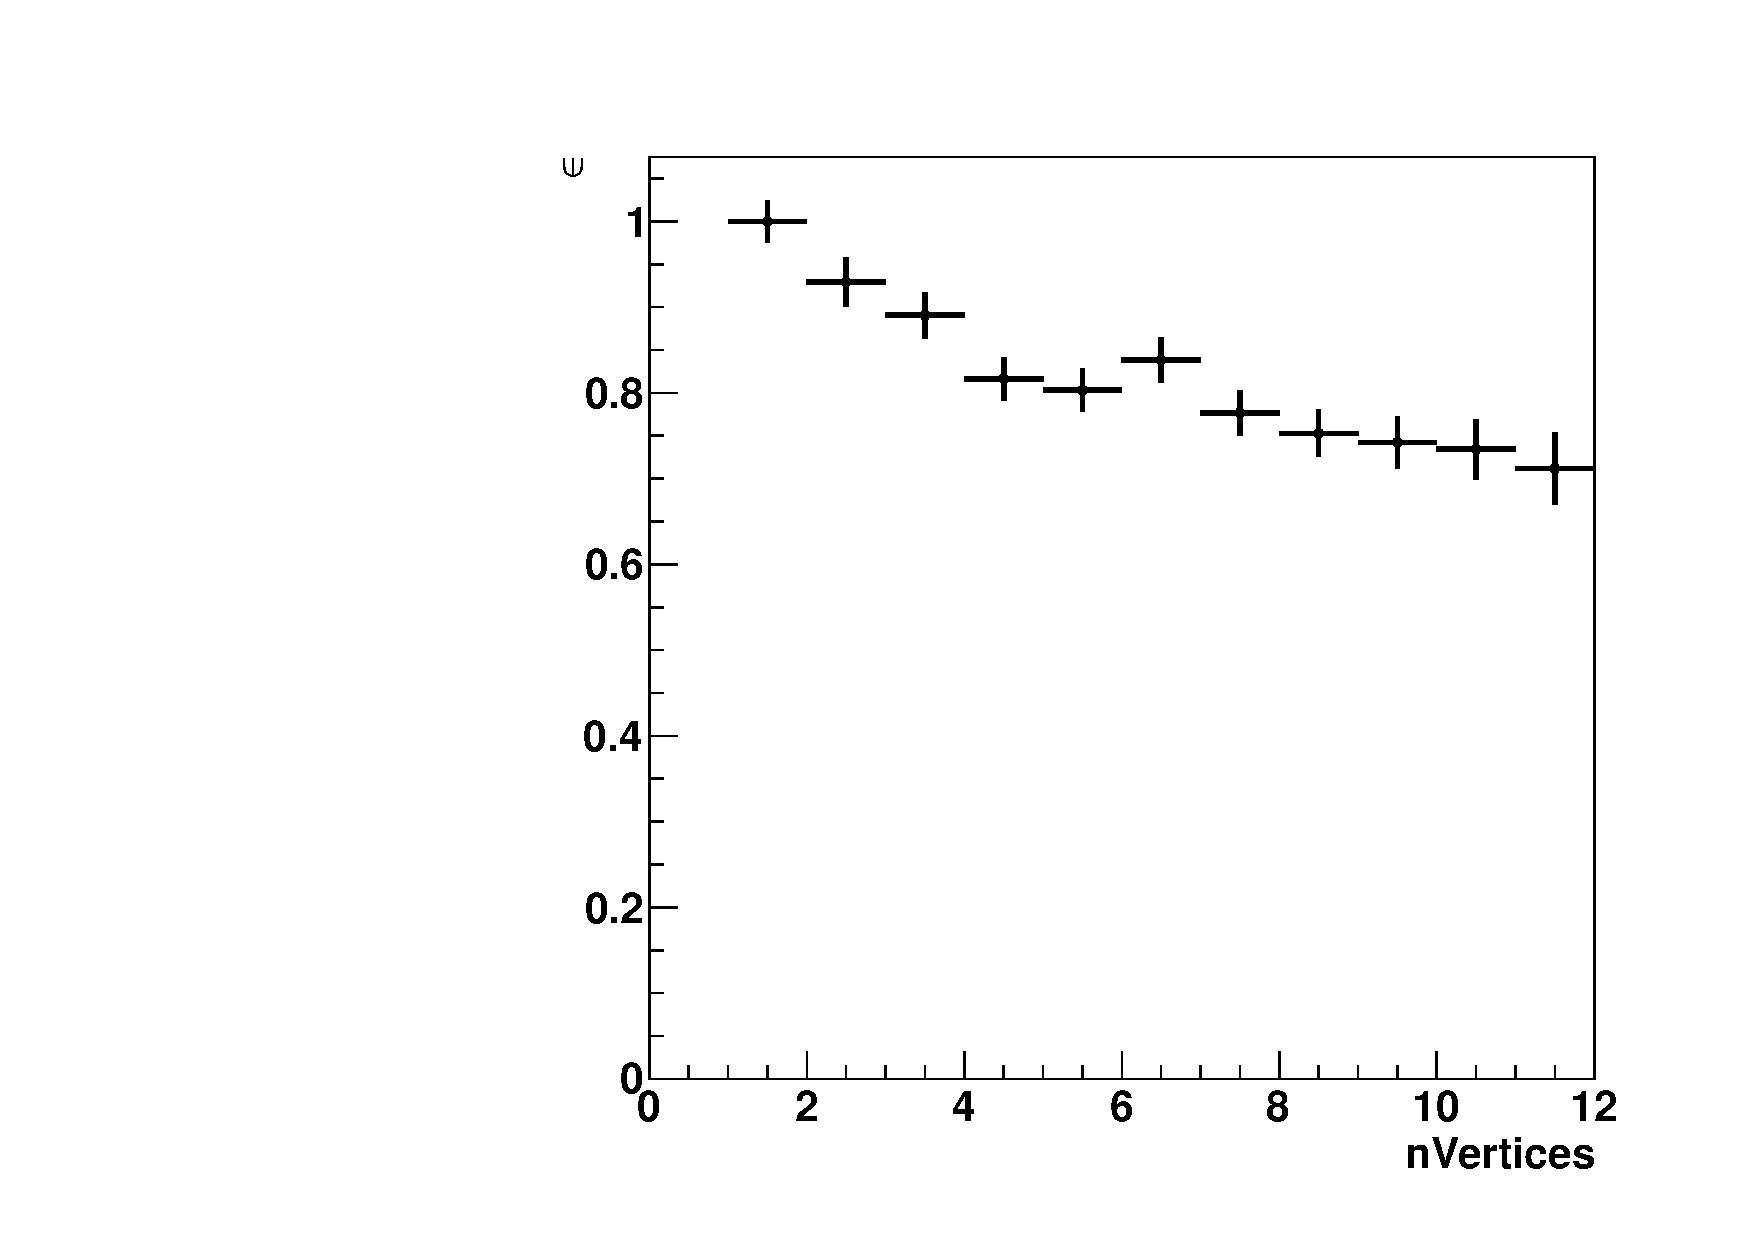
\includegraphics[width=0.7\textwidth]{Efficiency_vs_nVertices.pdf}
\end{center}
\caption{The relative photon efficiency as a function of the number of primary 
vertices.}
\label{fig:Efficiency_vs_nVertices}
\end{figure}

\begin{figure}
\begin{center}
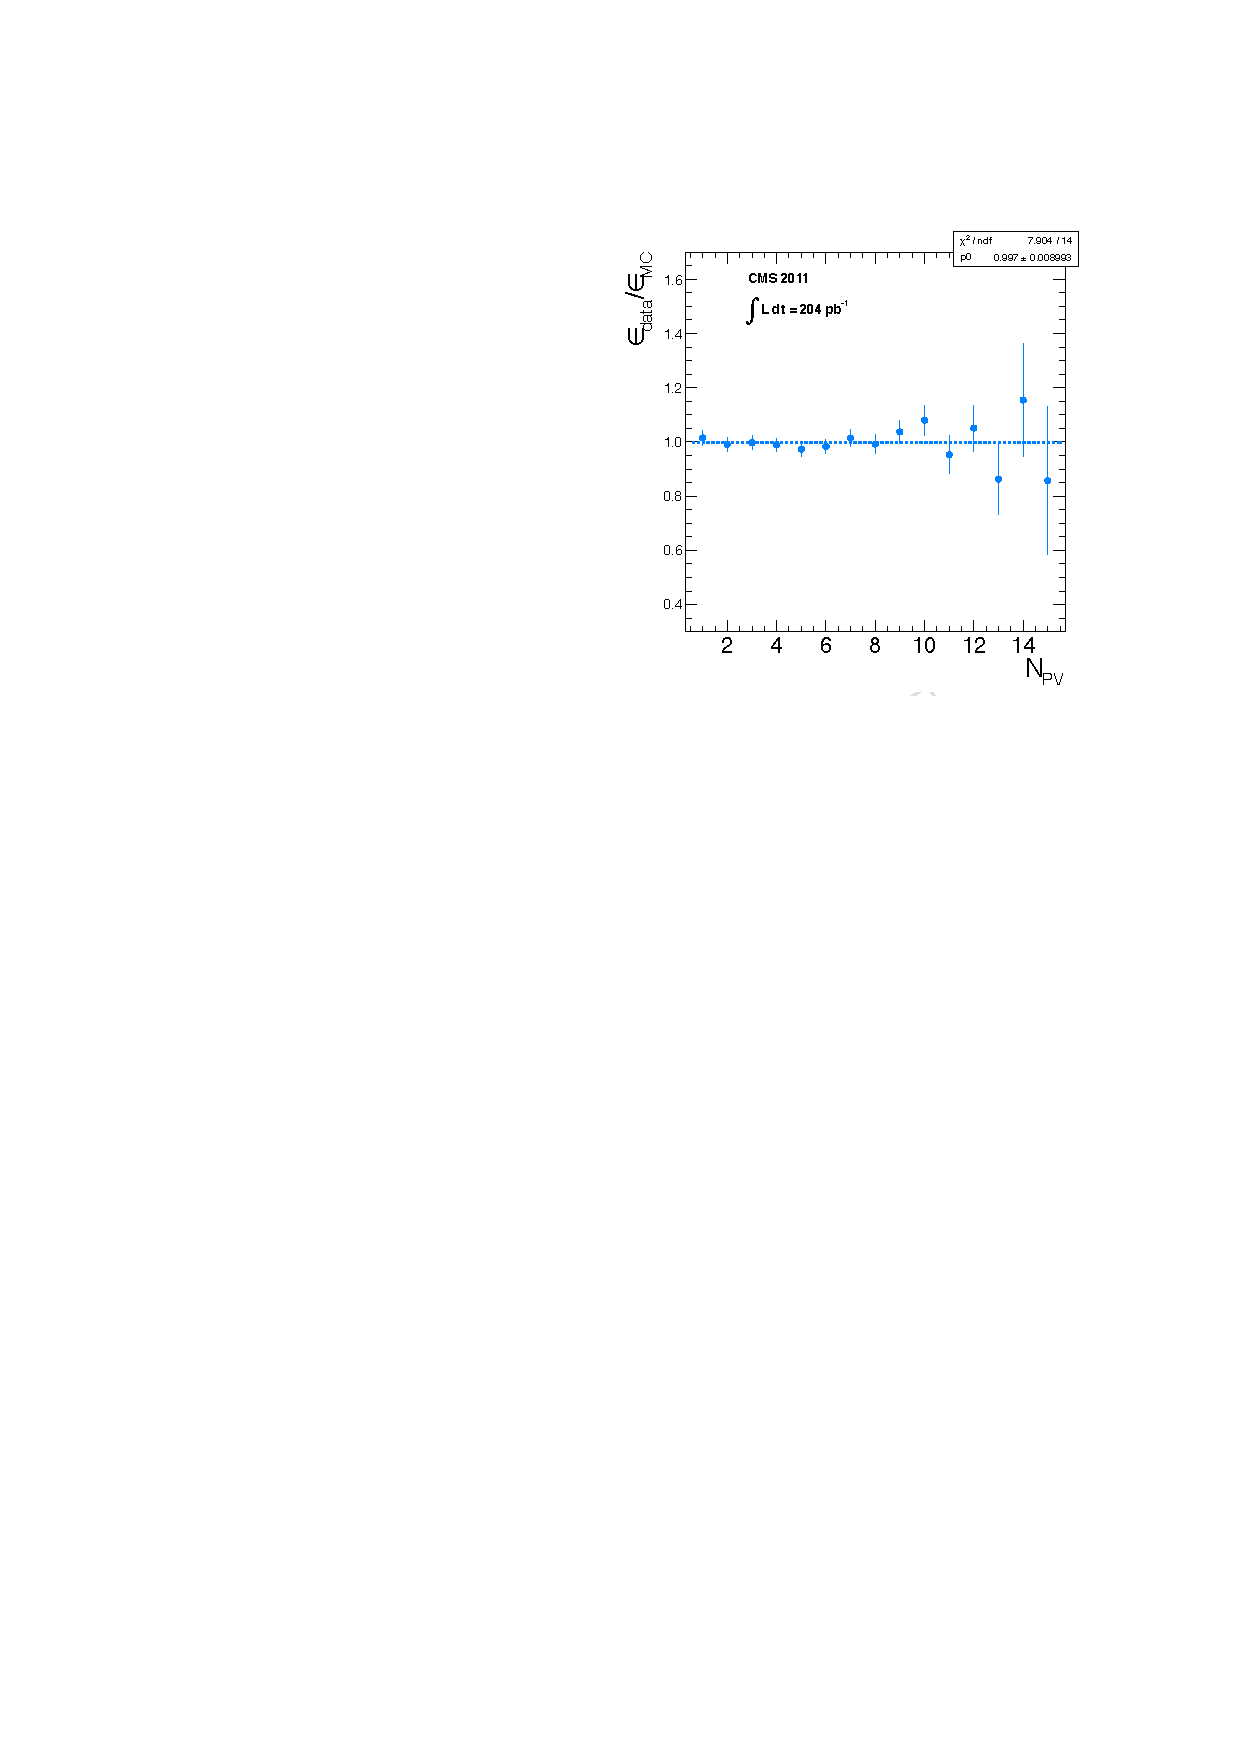
\includegraphics[width=0.7\textwidth]{EffCorr_vs_nPV.pdf}
\end{center}
\caption{The efficiency correction between data and MC as a function of the
number of primary vertices.}
\label{fig:EffCorr_vs_nPV}
\end{figure}

\begin{figure}
\begin{center}
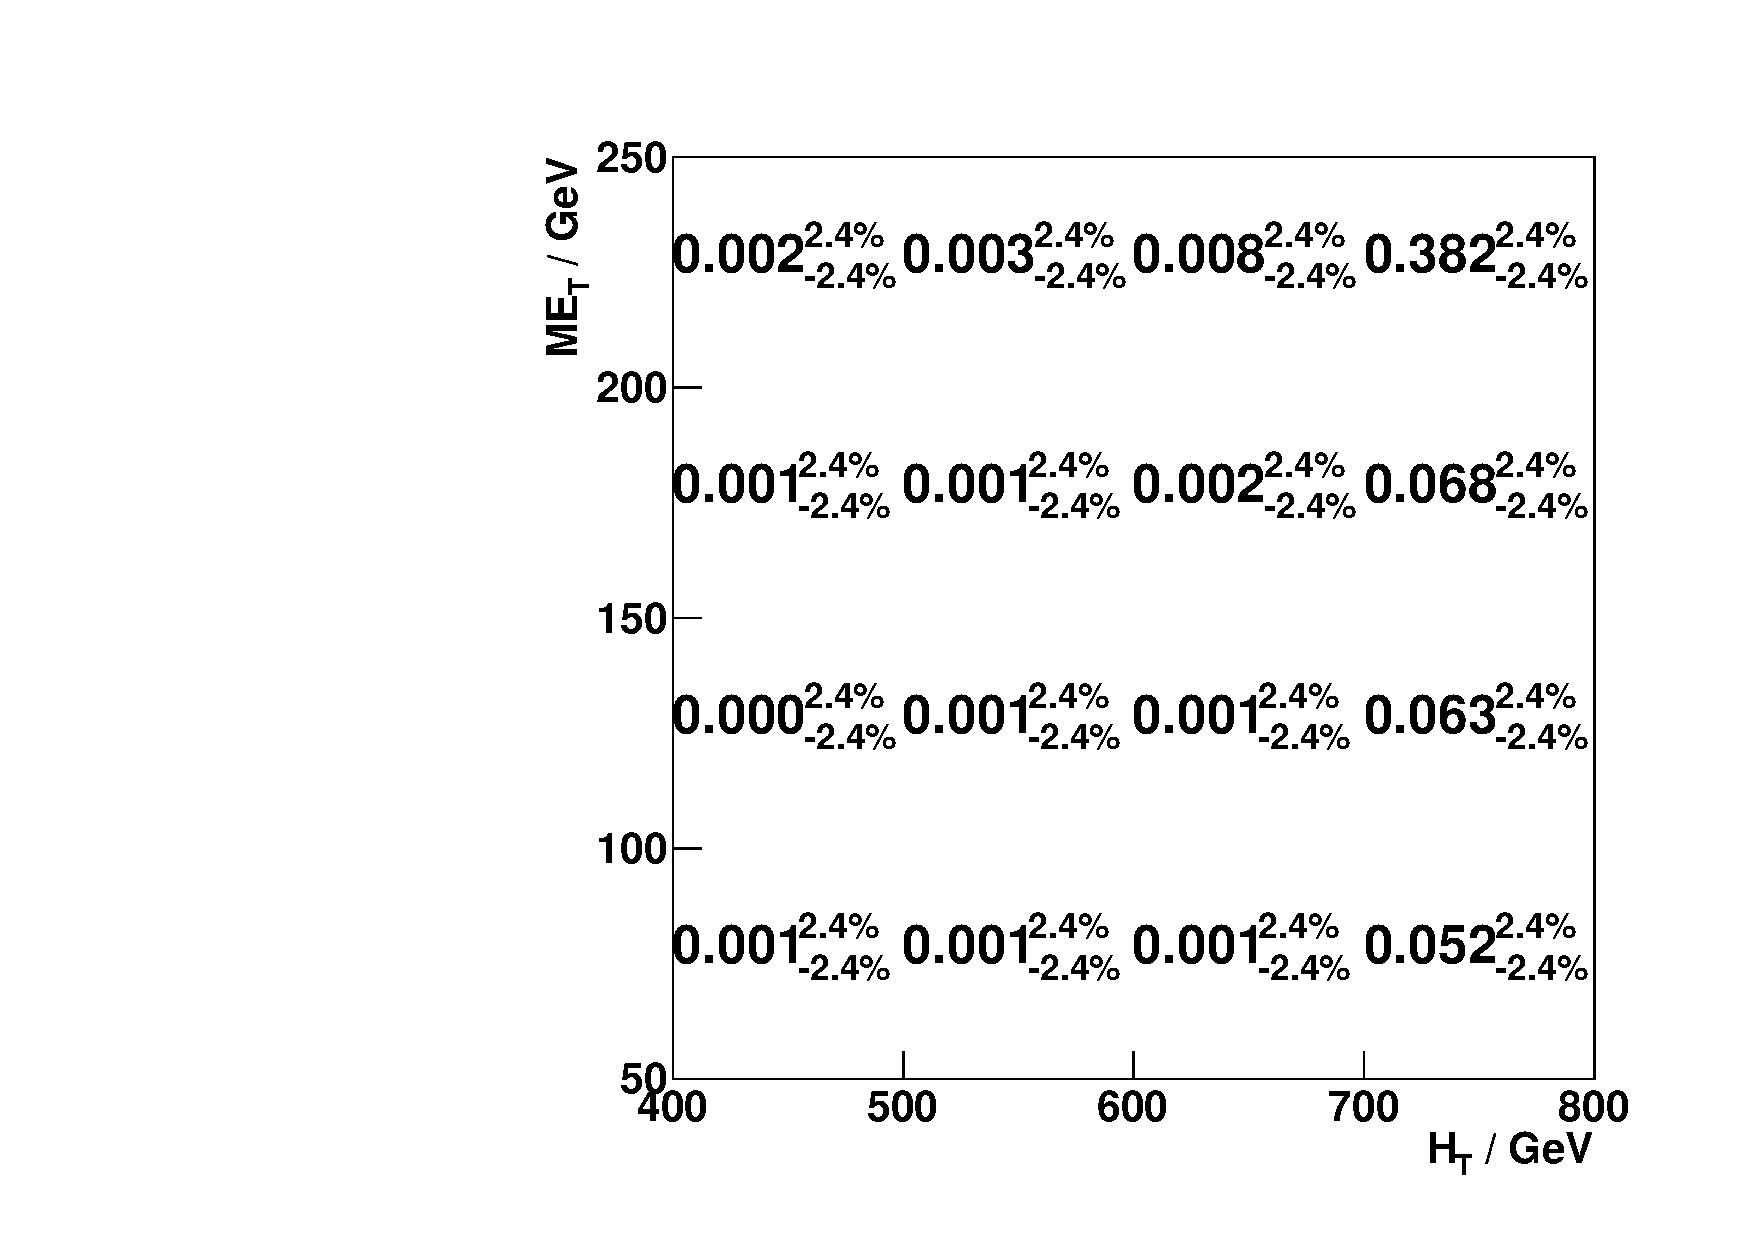
\includegraphics[width=0.7\textwidth]{SUSY_150_1040_1200_phoeff.pdf}
\end{center}
\caption{The percentage change in the signal efficiency when the photon
efficiency under pile-up is varied within its uncertainty.} 
\label{fig:phoeff_Numbers}
\end{figure}

\section{Signal Cross-Section}

Write how the cross-section is calculated. \\

There is a theoretical uncertainty on the signal cross-section due to the
uncertainty on the PDF distributions. Figure \ref{fig:xsec_unc} shows the
percentage uncertainty on the cross-section for each parameter point in the
mSquark vs mGluino plane.

\begin{figure}
\begin{center}
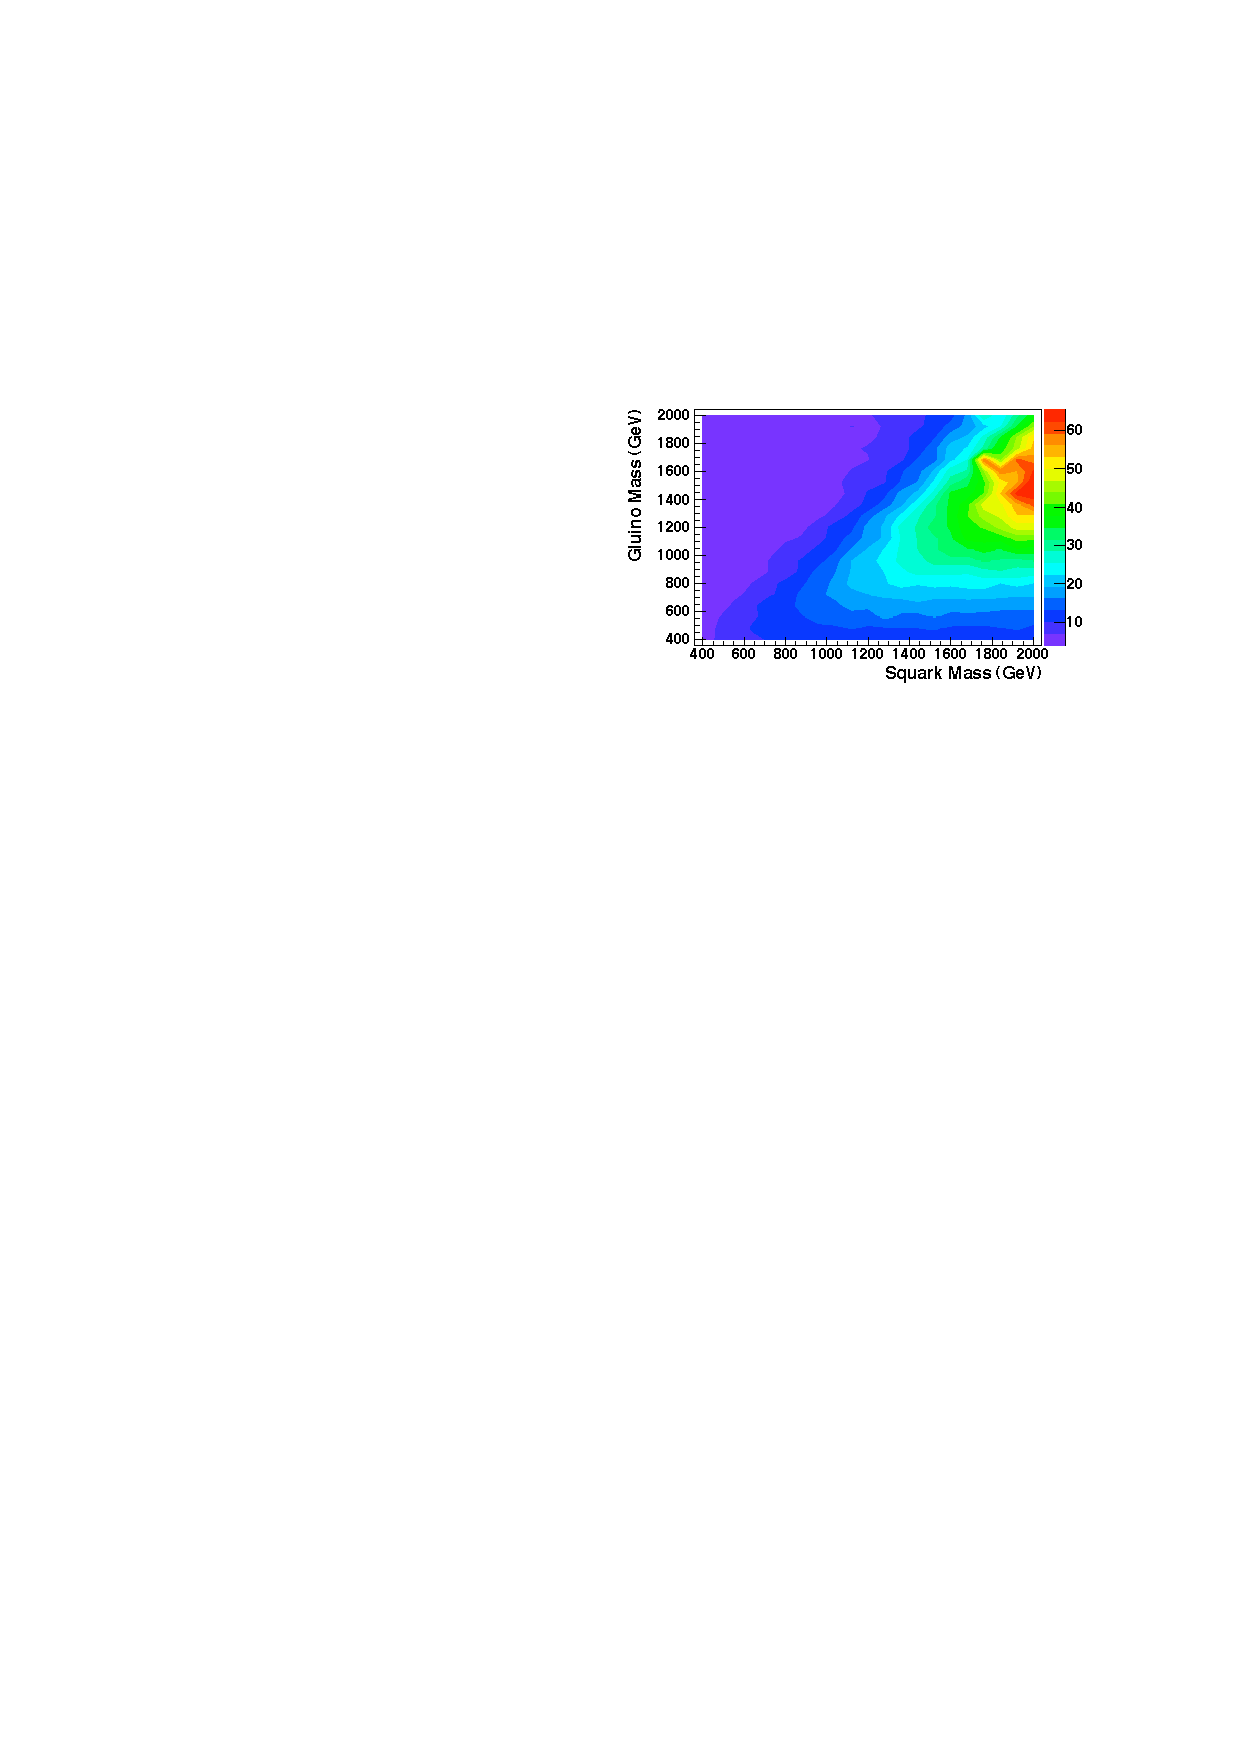
\includegraphics[width=0.7\textwidth]{Cross_Section_Uncertainty.pdf}
\end{center}
\caption{The percentage uncertainty on the signal cross-section based on PDF
uncertainties for each parameter point in the mSquark vs mGluino plane. 
Reproduced from \cite{ra3}.}
\label{fig:xsec_unc}
\end{figure}

\section{Integrated Luminosity}

There are a number of different ways of measuring the LHC luminosity. The method
used for early data was to use LHC beam parameters. The luminosity is given by:

\begin{equation}
L = \frac{N^{2}n_{b}f}{A_{eff}}
\label{eq:lumi}
\end{equation}

where N is the number of particles in each of the colliding bunches, $n_{b}$ is
the number of bunches, f is the revolution frequency of the beams and $A_{eff}$
is the effective transverse area in which the collisions occur. \\

The revolution frequency and the number of bunches are known precisely (to $\sim
1\%$) from measurements of the beam current. The limiting uncertainty for the
luminosity measurement is that of $A_{eff}$. The beam sizes must be controlled 
to 20-30\% for safe operation of the LHC. $A_{eff}$ is measured using van der 
Meer scans of the transverse beam profile \cite{vdm_scans}. Assuming a gaussian
transverse beam profile, $A_{eff}$ can be calculated as $A_{eff} = 
4\pi\sigma_{x}\sigma_{y}$. The uncertainty on the integrated luminosity 
measurement for this method is $10\%$. \\

The measurement can be improved using TOTEM and W/Z leptonic decays as standard
candles. TOTEM is a forward detector 240m from the interaction point designed to
measure the total proton-proton cross-section. By monitoring the cross-section
over time the integrated luminosity can be estimated. There are still acceptance
and PDF uncertainties associated with the cross-section measurement but these 
give a much smaller error on the integrated luminosity. The uncertainty from
this method is $4\%$.

\section{Summary of Systematics}

Table \ref{tab:Systematics_Summary} shows a summary of all the systematic
uncertainties for the backgrounds and the signal. For simplicity the systematic
uncertainties for only the most significant bin in terms of the limit setting 
($\HT$, $\MET$) = (700+, 200+) are shown.

\begin{table}
\begin{center}
\begin{tabular}{|c|c|c|c|}
\hline
{\bf Source of Systematic Uncertainty} & {\bf QCD} & {\bf EWK} & {\bf SUSY} \\
\hline
QCD Background Estimation & 5\% & - & - \\
\hline
e/$\gamma$ Misidentification & - & 30\% & - \\
\hline
$W\rightarrow e\nu$ Cross-Section & - &  & - \\
\hline
Photon Efficiency & - & 3.8\% & 3.8\% \\
\hline
Jet Energy Scale & - & & 4.4\% \\
\hline
Jet Energy Resolution & - & & 0.1\% \\
\hline
Pile-up: HT shift & - & & 0.1\% \\
\hline
Pile-up: MET smearing & - & & 0.0\% \\
\hline
Pile-up: photon efficiency & - & & 2.4\% \\
\hline
Signal Cross-Section & - & - & 20\% \\
\hline
Integrated Luminosity & - & 5\% & 5\% \\
\hline
\end{tabular}
\end{center}
\caption{A summary of the systematic uncertainties and how they affect the
expected number of events in the signal and each of the backgrounds.}
\label{tab:Systematics_Summary}
\end{table}
